\section{Introduction}

"Every day, nearly 400,000 babies are born around the world. None of them get to choose their gender, race, place of birth, or the social and economic conditions of their families. Life’s starting point is a lottery. But the future needn’t be left to chance," said Kristalina Georgieva, Chief Executive Officer of the World Bank, in their report on global intergenerational mobility \citep{narayan2018fair}. All parents, but especially those in the poorest segments of society in low-income countries, hope their children will have a better life than they have. And every child in those circumstances aspires to social mobility -- to break free from the constraints imposed by their birth. This idea was once called the "American Dream," but the ideal has long transcended American borders, instilling hope in children struggling in poverty around the world. A more precise term for it is intergenerational mobility. However, a dream is just a dream when, as the World Bank report shows, upward mobility remains elusive for the poor, especially in developing countries \citep{narayan2018fair}. Even in the so-called "land of opportunity," the U.S., opportunities for social mobility are not evenly distributed, as \citet{chetty2014land} has pointed out. This raises the question: Is our current progress fair? -- the very theme of the report mentioned above \citep{narayan2018fair}. It also reinforces the call for equality of opportunity, as existing inequalities deepen disparities and suppress mobility, a pattern captured by what we now call the "Great Gatsby curve."

People advocate for equality of opportunity to promote social mobility. But what does equality of opportunity truly mean? Should socioeconomic outcomes be entirely independent of parental status, ensuring complete social fluidity? This notion aligns with Nobel laureate Amartya Sen’s concept of development as freedom\nocite{sen2000development}. However, true freedom must also be accompanied by capability. Consider a country where relative educational mobility -- the extent to which a child's outcome depends on their parents -- is high. If much of this mobility results from downward movement, high social fluidity does not necessarily indicate progress. This highlights a key limitation: social fluidity does not always equate to social advancement, a challenge we term \textit{the directionality problem}. Another concern relates to absolute mobility, which attempts to measure whether children attain higher education levels than their parents. Although this measure considers \textit{the ceiling problem} -- the fact that children of the most educated parents cannot move upward -- it still oversimplifies progress. For instance, two countries may report similar upward mobility rates, but in one, progress stems from children of the least-educated families reaching higher levels, while in the other, mobility occurs mainly within well-educated groups. This reflects \textit{the difficulty problem}: current metrics flatten varying degrees of effort and structural constraints into a single value. Local measures that focus on the least advantaged can inform distributional concerns in line with Rawlsian principles \citep{Rawls1971}, but they are less effective in advanced countries where most individuals are already highly educated. Together, the directionality problem and the difficulty problem call into question how social mobility is currently measured.

To address these two problems, we develop a more comprehensive index to assess social progress in education using transition matrices, a method initially developed by \citet{prais1955measuring}, \citet{bibby1975methods}, and \citet{Bartholomew1967}. Firstly, we construct a target transition matrix representing the ideal educational progress that countries should achieve over time. The gap between actual and expected transition matrices is then measured. This approach accounts for country-specific factors, such as institutional and cultural contexts, ensuring that each country’s expected outcomes align with its initial educational distribution from the parent generation. By doing so, the measured gap reflects social progress while filtering out persistent factors like cultural norms or institutional constraints. More precisely, our index captures a country’s effort to improve social progress in education. While the expected matrices are country-specific, they follow a common underlying rule, aligning different countries to a shared reference frame for meaningful comparison. However, the validity of the index may be reduced in contexts affected by diploma inflation or shifts in educational quality, where formal attainment no longer reflects substantive progress. Despite this limitation, this new measure offers a more rigorous assessment of educational social progress, as it better reflects national efforts to enhance social mobility through education policies, independent of time-invariant country-specific contexts. Consequently, this study contributes to the measurement of global sustainable development goals.

The next section (Section \ref{sec:current}) reviews existing measures of social mobility, primarily from the World Bank, while also incorporating recent developments in the field. It concludes by highlighting the gap between the desired measurement of social progress and the challenges posed by the difficulty and directionality problems. Section \ref{sec:new} then details the construction of a novel approach to address this gap. This methodology is applied to the recently released global database on intergenerational mobility from the World Bank, demonstrating how our index better captures social progress compared to existing measures (see Section \ref{sec:application}). The paper concludes with a discussion of its contributions to the field and potential directions for future research (see Section \ref{sec:conclusion}).



\section{Current measures of social mobility} \label{sec:current}

Social mobility is commonly measured using three approaches \citep{blanden2013cross}: ordinal transition matrices (education), continuous measures (earnings), and categorical measures (occupations). Earnings-based measures, such as intergenerational elasticity (IGE), provide numerical precision but are highly volatile due to career shifts, economic fluctuations, and exogenous shocks. Moreover, tracking income across generations requires reliable longitudinal data, which is often unavailable. Occupational measures, while easier to collect, lack strict hierarchical ordering and face classification inconsistencies across countries, making cross-national comparisons challenging. Education-based transition matrices provide a more stable and structured method for analyzing intergenerational mobility. Educational attainment is widely accessible, less prone to short-term fluctuations, and offers a clear, ordered ranking that corresponds with social stratification. This enables a systematic evaluation of mobility patterns across generations. Education-based measures are frequently used for global comparisons due to their reliability and comparability due to its uniform international classification (ISCED). Although these matrices may be less effective in cases of diploma inflation or changes in educational quality, they remain one of the most reliable indicators of intergenerational mobility, effectively capturing the persistence of social status across generations.

\paragraph{Common measures}  

Intergenerational mobility in education can be assessed through two key concepts: absolute mobility and relative mobility. This study primarily adopts the World Bank’s approach \citep{van2024intergenerational, narayan2018fair} to intergenerational mobility (as shown in Table \ref{tab:measures}). Absolute mobility measures the proportion of individuals who achieve a higher education level than their parents. Two key indicators for this are \textit{CAT}, which calculates the probability that a child surpasses their parents’ education level assuming the parents did not complete university, and \textit{MIX}, which includes both children who exceed their parents' education and those who reach university if at least one parent did. In contrast, relative mobility focuses on how much a child’s education is influenced by their parents’ education. The lower the dependency on parents' education, the higher the relative mobility. This is often measured with statistical indicators such as \textit{1-COR}, which calculates one minus the correlation between parents’ and children’s years of schooling, and \textit{1-BETA}, which is derived from a regression model predicting a child’s years of schooling based on their parents' years of schooling. Both of these metrics suggest that higher values indicate greater mobility. Additionally, several measures specifically focus on mobility for children from disadvantaged backgrounds. \textit{MU050} estimates the expected education level of a child whose parents are in the bottom half of the education distribution. \textit{BHQ4} measures the likelihood that a child from a low-education family reaches higher education levels, while \textit{AHMP} tracks the percentage of children who complete primary school when neither parent has done so.

\begin{table}[h!]
    \centering
 
    \caption{Common measures of intergenerational mobility}
    \renewcommand{\arraystretch}{1.5}
  	\resizebox{1\textwidth}{!}{
    \begin{tabular}{|m{0.12\textwidth}|m{0.6\textwidth}|m{0.4\textwidth}|}
    \hline
    \centering \textbf{Metrics} & \centering \textbf{Explain} & \centering \textbf{Formula} \tabularnewline
    \hline
    \centering CAT & \raggedright Pr child surpasses parent’s educational category (conditional on parent not having tertiary) & \centering
    \begin{equation*}
    \operatorname{Pr}[ R_{c}  >R_{p} |R_{p} < 5]
    \vspace{-1em}\end{equation*} \tabularnewline
    \hline
    \centering MIX & \raggedright Share of respondents with strictly higher educational category than parents if parents do not have tertiary, or with tertiary education if either parent has tertiary. & \centering
    \begin{equation*}
    \operatorname{Pr}[( R_{c}  >R_{p}) \cap ( R_{c} =R_{p} =5)]
    \vspace{-1em}\end{equation*} \tabularnewline
    \hline
    \centering 1-COR & \raggedright 1 minus the correlation coefficient between respondents' and parents' years of schooling. & \centering
    \begin{equation*}
    1-\frac{\operatorname{Cov}( Y_{c} ,Y_{P})}{\sqrt{\operatorname{Var}( Y_{c}) \times \operatorname{Var}( Y_{P})}}
    \vspace{-1em}\end{equation*} \tabularnewline
    \hline
    \centering 1-BETA & \raggedright 1 minus the coefficient from regressing respondents' years of schooling on parents' years of schooling. & \centering
    \begin{equation*}
    1-\frac{\operatorname{Cov}( Y_{c} ,Y_{P})}{\operatorname{Var}( Y_{P})}
    \vspace{-1em}\end{equation*} \tabularnewline
    \hline
    \centering MU050 & \raggedright Expected child educational rank from a person born in bottom half & \centering
    \begin{equation*}
    \operatorname{\mathbb{E}}[ R_{c} |R_{p} < Q_{2}]
    \vspace{-1em}\end{equation*} \tabularnewline
    \hline
    \centering BHQ4 & \raggedright Pr child from bottom half reaches top quartile & \centering
    \begin{equation*}
    \operatorname{Pr}[ R_{c}  >Q_{3} |R_{p} < Q_{2}]
    \vspace{-1em}\end{equation*} \tabularnewline
    \hline
    \centering AHMP & \raggedright Share of respondents with a completed primary education conditional on neither parent having completed primary education. & \centering
    \begin{equation*}
    \operatorname{Pr}[ R_{c} \geq 2|R_{p} < 2]
    \vspace{-1em}\end{equation*} \tabularnewline
    \hline
    \end{tabular}
}
    \vspace{0.2cm}
    \label{tab:measures}
    \captionsetup{font=footnotesize}
    \caption*{\textbf{Notes:} \( c \) denote the child and \( p \) denote the parent. The variable \( Y \) represents years of schooling, while education levels are categorized as \( R = \{1,2,3,4,5\} \), corresponding to (1) less than primary, (2) primary, (3) lower secondary, (4) upper secondary, and (5) tertiary education. The second and third quartiles of the education distribution are denoted as \( Q_2 \) and \( Q_3 \), respectively.\\
    Source: adapted from \citet{van2024intergenerational}}
\end{table}


\paragraph{Other measures}

There are additional measures beyond those mentioned above, which have been adopted by the World Bank, but they are less commonly used for comparing social progress across countries. The Prais-Bibby index \citep{bibby1975methods, prais1955measuring} quantifies mobility by measuring the proportion of individuals who change ranks between generations, providing a straightforward approach to assessing relative mobility. The Bartholomew index \citep{Bartholomew1967} focuses on movement between ordered categories, particularly in education, calculating the weighted average distance moved between parental and children's categories. Its standardized version offers a clearer view of upward mobility. \citet{apouey2023ordinal} introduced an inequality-sensitive and additive achievement measure for ordinal data, which combines both average achievement and the inequality of achievement within a generation, offering a more nuanced perspective on mobility that accounts for both individual movement and societal inequality. The upward mobility kernel developed by \citet{ray2023measuring}, based on the principle of growth progressivity, provides a theoretical framework for measuring upward mobility by considering individual growth rates in relation to baseline income. Finally, entropy-based measures \citep{mueller2021entropy}, derived from information theory, evaluate how much a parent’s status reduces uncertainty about a child's future status. Higher information gain in this context suggests stronger intergenerational dependence and, consequently, higher immobility. Together, these indices and measures form a comprehensive toolkit for analyzing the complex dynamics of social mobility.

\paragraph{The big gap}

Nevertheless, there is a gap between current measures of social progress. The definition of social progress is broad, encompassing not only education and income but also health, well-being, and human rights \citep{narayan2018fair, blanden2013cross, deutscher2023measuring}. The focus here is not on defining social progress in its entirety but on highlighting how current measurements of social mobility do not fully capture social progress in education. While social progress in education can be closely linked to intergenerational mobility -- where each generation attains better education -- existing measures fail to capture social progress across countries. Consider two illustrative examples. First, a comparison between Bhutan and the Central African Republic (as shown in Figure \ref{fig:compare1}) reveals that their absolute mobility, measured by the indices \textit{CAT} and \textit{MIX}, is nearly identical. However, the Central African Republic exhibits significantly higher relative mobility, as indicated by $1 - BETA$ (0.53 vs. 0.21 for Bhutan). Based on this, one might conclude that the Central African Republic has achieved greater social progress than Bhutan. However, looking at their transition matrices reveals a different story. The Central African Republic has higher relative mobility primarily due to widespread downward mobility -- for instance, over 35\% of individuals with parents who attained at least primary education have themselves remained below the primary level ($C_1P_2 + C_1P_3 > 35\%$). This example demonstrates that social fluidity does not necessarily translate into progress. This issue is referred to as the \textit{directionality problem}. The directionality problem is not only about distinguishing upward from downward mobility but also about considering intergenerational persistence (social stagnation), which is less concerning than downward mobility. In Bhutan’s case, persistence is high. However, this is preferable to the higher prevalence of downward mobility seen in the Central African Republic.

\begin{figure}[!ht]
    \centering
    \scalebox{0.55}{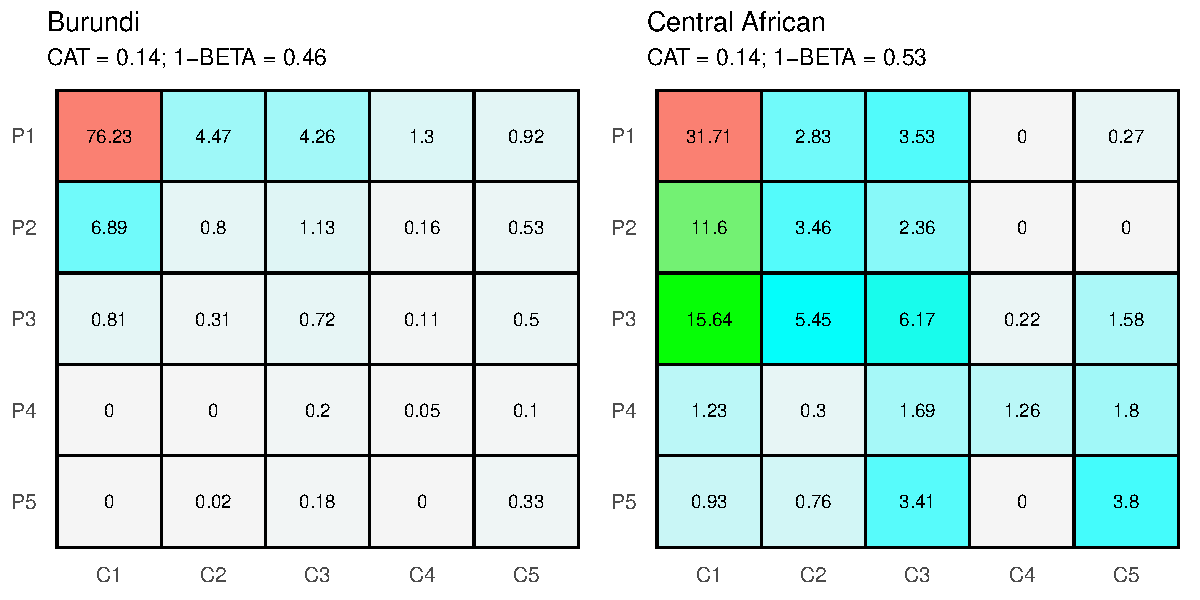
\includegraphics{figs/compare1.pdf}}
    \caption{Absolute Mobility Comparison}
    \label{fig:compare1}
    \captionsetup{font=footnotesize}
    \caption*{\textbf{Notes:} \textit{CAT} measures absolute mobility, \textit{1-BETA} measures relative mobility. The data is sourced from the Global Database on Intergenerational Mobility (2023). The analysis focuses on the 1980 cohort, comparing the education levels of all children to the maximum education level of their parents.}
\end{figure}

The second example compares Canada and Timor-Leste (as shown in Figure \ref{fig:compare2}), where Canada exhibits higher absolute and relative mobility. However, can one conclude that Canada has made more progress than Timor-Leste? Examining their transition matrices suggests otherwise. It would be unfair to say that Timor-Leste has made less progress simply because its mobility primarily comes from disadvantaged groups, whereas mobility in Canada occurs mostly among the upper class. The effort required to achieve mobility in these two contexts is vastly different. More than a quarter of Timor-Leste’s population, whose parents had less than primary education, managed to move up to the upper secondary or tertiary level, indicating a significant achievement. In contrast, mobility in Canada mostly involves individuals moving from upper secondary to tertiary education, which represents a smaller feat in comparison. This issue is referred to as the \textit{difficulty problem}, as different social classes face different levels of difficulty in achieving the same educational outcome. For example, the hurdle of intergenerational transition from $P_1$ to $C_5$ is higher than that from $P_4$ to $C_5$. Notably, \textit{CAT} does not account for individuals whose parents had tertiary education, and \textit{MIX} treats cases where both parents and children attain the highest education level ($C_5P_5$) as upward mobility is restricted due to ceiling effects.

\begin{figure}[!ht]
    \centering
    \scalebox{0.55}{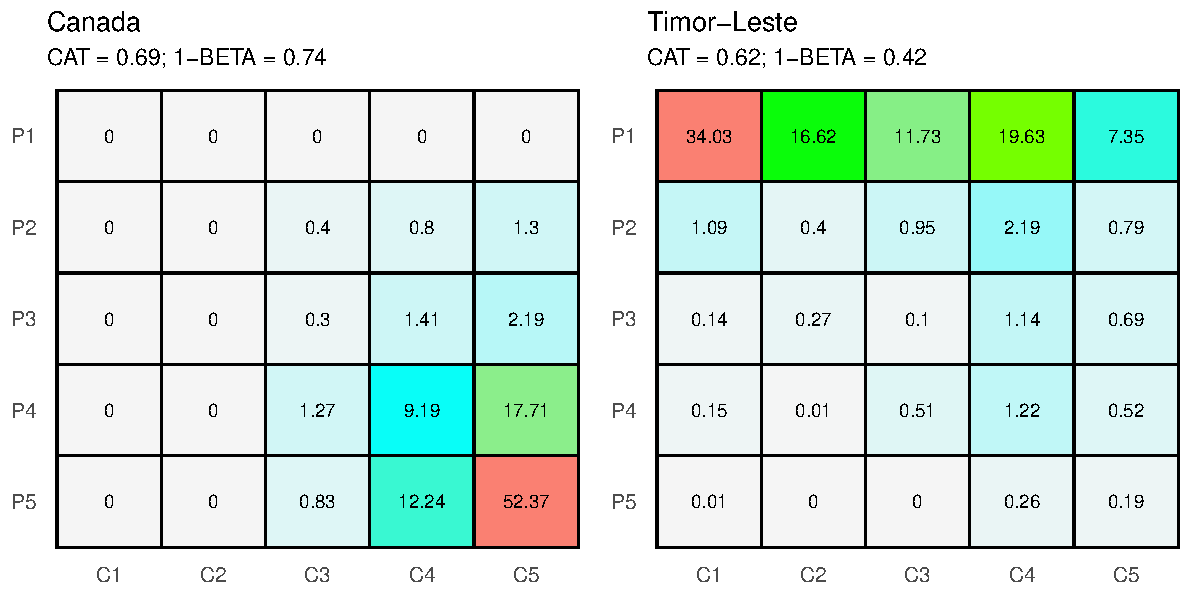
\includegraphics{figs/compare2.pdf}}
    \caption{Relative Mobility Comparison}
    \label{fig:compare2}
    \captionsetup{font=footnotesize}
    \caption*{\textbf{Notes:} \textit{CAT} measures absolute mobility, \textit{1-BETA} measures relative mobility. The data is sourced from the Global Database on Intergenerational Mobility (2023). The analysis focuses on the 1980 cohort, comparing the education levels of all children to the maximum education level of their parents.}
\end{figure} 

\textit{In summary}, current measures of social mobility are inadequate for assessing social progress in education. They also do not allow for a straightforward comparison between countries. Although local measures can be helpful, they cannot capture a comprehensive picture of social progress. Therefore, we developed a more comprehensive index to evaluate the social progress of education using transition matrices. This approach functions like a dimensionality reduction method that condenses information into a single uni-dimensional measure. However, this measure provides far more insight into social progress than conventional dimensionality reduction techniques.. The proposed methodology directly addresses the difficulty and directionality problems outlined above. In the following section, a target transition matrix is constructed to represent the ideal educational progress countries should achieve over time. The gap between the actual and expected transition matrices is then measured. This method accounts for country-specific backgrounds (such as institutional and cultural factors), ensuring that each country’s expected outcomes align with its initial educational distribution from the parent generation. By doing so, the gap reflects social progress while eliminating differences that are relatively stable over time, such as cultural norms or institutional constraints. More precisely, our index measures the country's effort to obtain social progress in terms of education. Importantly, while the expected matrices are country-specific, they follow a common underlying rule -- similar to aligning different countries to a shared reference frame for meaningful comparison.

\section{A new measure of social progress} \label{sec:new}

As discussed in the previous section, we define the expected transitions matrix to compute the gap between the actual matrix and the expected one, measuring the social progress gap via education. An expected transitions matrix must address both the difficulty and directionality problems while remaining country-specific to eliminate unobserved fixed effects such as culture and institutions. Therefore, we start with the original education distribution of the parent generation, where \( P_1 \) is the probability of a parent having education level 1, \( P_2 \) for level 2, \( P_3 \) for level 3, \( P_4 \) for level 4, and \( P_5 \) for level 5. Our goal is to establish the destination education distribution of the child generation while preserving the original distribution. In other words, the row sums of the expected matrix at each parent education level must equal those of the actual matrix:  
\begin{equation}
\sum_{i=1}^{5} \operatorname{Pr}[R_c = i, R_p = j] = \operatorname{Pr}[R_p = j] = P_j.
\label{eq:1}
\end{equation}

\paragraph{The directionality problem}
To address the directionality problem, we divide the expected matrix into three areas: downward, persistent, and upward (see Table \ref{tab:matrix}). Since the expected matrix reflects the desired pattern of social mobility, the downward area should be zero (as there is no social progress involved in downward mobility), the persistent area should be minimized (but remain greater than zero, as it is not as undesirable as downward mobility and is an inevitable part of social mobility), and the remaining probabilities should be allocated to the upward region. There are two major issues to resolve here. First, we must determine the minimum extent of the intergenerational transmission. As discussed earlier regarding the ceiling effect, when parents have the highest education level, their children have no possible space for upward mobility. Therefore, this case cannot be treated the same as other persistent cases. In the expected matrix, children should retain their parents' highest education level, meaning  
\[
\operatorname{Pr}[R_c=5, R_p=5]=\operatorname{Pr}[R_p=5]=P_5.
\]
For other cases in the persistent area, an intergenerational transmission effect of education is assumed, recognizing that parenting itself serves as a form of education. However, the genetic lottery is not expected to influence educational outcomes. In terms of equality of opportunity, as defined by \citet{roemer2015equality}, luck -- such as the genetic lottery -- should be independent of outcomes. Based on evidence on the causal effect of intergenerational transmission (which isolates genetic transmission from education attainment), we assume a true intergenerational effect of \(\omega=0.1\) following \citet{holmlund2011causal}. This implies that there is a 10\% probability that children remain at the same education level as their parents:  
\[
\operatorname{Pr}[ R_{c} =i, R_{p} =i] =\omega \operatorname{Pr}[ R_{p} =i],\ \forall \ i< 5.
\]

We recognize that our method is sensitive to the choice of \(\omega\). To assess robustness, we conducted an additional calculation with \(\omega = 0.15\), following \citet{fleury2018intergenerational}, and found that the results remain stable (see \ref{app:sensitive}). One could argue for using \(BETA\) values from each country or the mean of \(BETA\) across countries as persistent probabilities instead of our approach. However, using country-specific \(BETA\) values would not produce a comparable index. In countries with high actual persistence, such as Bhutan, the difference between the expected and actual matrices would be small, making it impossible to conclude whether Bhutan is progressive. While the mean \(BETA\) across countries might better measure progress, it does not address the problem of the genetic lottery, which is a barrier to equality of opportunity. Moreover, \(BETA\) is derived from actual values, whereas an expected matrix should be defined independently of actual values to properly measure progress. 
Therefore, setting a fixed intergenerational effect makes more sense as a shared reference frame. However, it remains subject to the original circumstances of each country since the persistent value is determined by the product of \(\omega\) and the original education distribution of the parent generation.

\paragraph{The difficulty problem}

The second major challenge lies in distributing the remaining probabilities into the upward area while adhering to the difficulty rule. To address this, we first establish assumptions for an ideal society that promotes social progress.

\begin{assumption} \label{assump:1}
Society should ensure that every child can achieve up to  an education level \( R_c \leq z \)  that is obtained by others  with the same background \( R_p = i \).
\[
\operatorname{Pr}(R_c = j, R_p = i \mid R_c = z, R_p = i) = 1, \forall j < z.
\]
\end{assumption}

\begin{assumption} \label{assump:2}
Society expects that children from better backgrounds (\( R_p > i \)) will achieve at least the same education level \( R_c = z \) as those from disadvantaged backgrounds (\( R_p < j \)).
\[
\operatorname{Pr}(R_c = z, R_p = j \mid R_c = z, R_p = i) = 1, \forall i < j.
\]
\end{assumption}

From Assumptions \ref{assump:1} and \ref{assump:2}, we can infer:

\begin{equation} \label{eq:2}
\begin{array}{l}
\operatorname{Pr}(R_c = z, R_p = j \cap R_c = j, R_p = i \mid R_c = z, R_p = i) = 1 \\
\Rightarrow \operatorname{Pr}(R_c = j, R_p = j \mid R_c = z, R_p = i) = 1
\end{array}
\end{equation}

This implies that if children have experienced significant upward mobility (e.g., from \( i \) to \( z \)), others should also be able to achieve mobility within the range from \( i \) to \( z \). This includes the possibility of intergenerational persistence, where children are able to remain in the same social class as their parents \( i \).

\begin{assumption} \label{assump:3}
The chances of achieving education for individuals on different, non-overlapping social mobility paths (e.g., from level \( i \) to \( j \) versus from \( j \) to \( z \)) are independent of each other.
\[
\operatorname{Pr}(R_c = j, R_p = i \mid R_c = z, R_p = j) = \operatorname{Pr}(R_c = j, R_p = i), \forall j < z.
\]
\end{assumption}

From Assumption \ref{assump:3}, we multiply both sides by \( \operatorname{Pr}(R_c = z, R_p = j) \):

\[
\begin{array}{l}
\operatorname{Pr}(R_c = j, R_p = i) \times \operatorname{Pr}(R_c = z, R_p = j) \\
= \operatorname{Pr}(R_c = j, R_p = i \mid R_c = z, R_p = j) \times \operatorname{Pr}(R_c = z, R_p = j) \\
= \operatorname{Pr}(R_c = j, R_p = i \cap R_c = z, R_p = j)
\end{array}
\]

Because of the commutative property of intersection in probability, the right-hand side can be rewritten as:

\[
\operatorname{Pr}(R_c = j, R_p = i) \times \operatorname{Pr}(R_c = z, R_p = j) = \operatorname{Pr}(R_c = j, R_p = j \cap R_c = z, R_p = i)
\]

By applying Equation~\eqref{eq:2} to this, we obtain:

\[
\operatorname{Pr}(R_c = z, R_p = i) = \operatorname{Pr}(R_c = z, R_p = j) \times \operatorname{Pr}(R_c = j, R_p = i).
\]
To operationalize this, let \( a \), \( b \), \( c \), and \( d \) represent the probabilities of transitioning from one education level to the next, in accordance with Assumption \ref{assump:3}, specifically: \( a = \operatorname{Pr}(R_c = 2, R_p = 1) \), \( b = \operatorname{Pr}(R_c = 3, R_p = 2) \), \( c = \operatorname{Pr}(R_c = 4, R_p = 3) \), and \( d = \operatorname{Pr}(R_c = 5, R_p = 4) \). Using these definitions, we express the expected transition matrix (see Table \ref{tab:matrix}) as follows:

% \usepackage{color}
% \usepackage{tabularray}
\definecolor{GoldenFizz}{rgb}{0.984,0.984,0.274}
\definecolor{SpringGreen}{rgb}{0.054,0.984,0.58}
\definecolor{Froly}{rgb}{0.952,0.447,0.447}
\begin{table}[H]
\centering
\caption{The expected matrix}
\label{tab:matrix}
\begin{tblr}{
  cells = {c},
  cell{2}{2} = {GoldenFizz},
  cell{2}{3} = {SpringGreen},
  cell{2}{4} = {SpringGreen},
  cell{2}{5} = {SpringGreen},
  cell{2}{6} = {SpringGreen},
  cell{3}{2} = {Froly},
  cell{3}{3} = {GoldenFizz},
  cell{3}{4} = {SpringGreen},
  cell{3}{5} = {SpringGreen},
  cell{3}{6} = {SpringGreen},
  cell{4}{2} = {Froly},
  cell{4}{3} = {Froly},
  cell{4}{4} = {GoldenFizz},
  cell{4}{5} = {SpringGreen},
  cell{4}{6} = {SpringGreen},
  cell{5}{2} = {Froly},
  cell{5}{3} = {Froly},
  cell{5}{4} = {Froly},
  cell{5}{5} = {GoldenFizz},
  cell{5}{6} = {SpringGreen},
  cell{6}{2} = {Froly},
  cell{6}{3} = {Froly},
  cell{6}{4} = {Froly},
  cell{6}{5} = {Froly},
  cell{6}{6} = {GoldenFizz},
  cell{7}{1} = {c=6}{},
  hlines,
  vlines,
}
            & \textbf{C1}                         & \textbf{C2}                         & \textbf{C3}                         & \textbf{C4}                          & \textbf{C5}                               & \textbf{Total}        \\
\textbf{P1} & $\displaystyle \omega \times P_{1}$ & $\displaystyle a$                   & $\displaystyle a\times b$           & $\displaystyle a\times b\times c$    & $\displaystyle a\times b\times c\times d$ & $\displaystyle P_{1}$ \\
\textbf{P2} & 0                                   & $\displaystyle \omega \times P_{2}$ & $\displaystyle b$                   & $\displaystyle b\times c$            & $\displaystyle b\times c\times d$         & $\displaystyle P_{2}$ \\
\textbf{P3} & 0                                   & 0                                   & $\displaystyle \omega \times P_{3}$ & $\displaystyle c$                    & $\displaystyle c\times d$                 & $\displaystyle P_{3}$ \\
\textbf{P4} & 0                                   & 0                                   & 0                                   & $\displaystyle \omega \times P_{4} $ & $\displaystyle d$                         & $\displaystyle P_{4}$ \\
\textbf{P5} & 0                                   & 0                                   & 0                                   & 0                                    & $\displaystyle P_{5}$                     & $\displaystyle P_{5}$ \\
            &                                     &                                     &                                     &                                      &                                           & \textbf{100\%}        
\end{tblr}
\vspace{0.2cm}
\captionsetup{font=footnotesize}
    \caption*{\textbf{Notes:} The upward area is colored green, the persistent area is colored yellow, and the downward area is colored red.}
\end{table}

Applying the law of total probability to this structure, the constraints on the transition probabilities can be written as:

\[
\begin{cases}
a + a \times b + a \times b \times c + a \times b \times c \times d = (1 - \omega) P_1 < 1, \\
b + b \times c + b \times c \times d = (1 - \omega) P_2 < 1, \\
c + c \times d = (1 - \omega) P_3 < 1, \\
d = (1 - \omega) P_4 < 1.
\end{cases}
\]
Solving for \( a \), \( b \), \( c \), and \( d \), we get:

\begin{equation}
\begin{cases}
\displaystyle a = \frac{(1 - \omega) P_1}{1 + (1 - \omega) P_2} < 1, \\
\displaystyle b = \frac{(1 - \omega) P_2}{1 + (1 - \omega) P_3} < 1, \\
\displaystyle c = \frac{(1 - \omega) P_3}{1 + (1 - \omega) P_4} < 1, \\
\displaystyle d = (1 - \omega) P_4 < 1.
\end{cases}
\label{eq:3}
\end{equation}
As shown in equation~\eqref{eq:3}, all transition probabilities are less than one, meaning the allocation of probabilities into the upward area remains valid. Figure~\ref{fig:VNM_USA} presents real examples from Vietnam and the United States using our method, with the left-side charts displaying the actual transition matrices and the right-side charts showing the expected matrices.

\begin{figure}[H]
    \centering
    \scalebox{0.55}{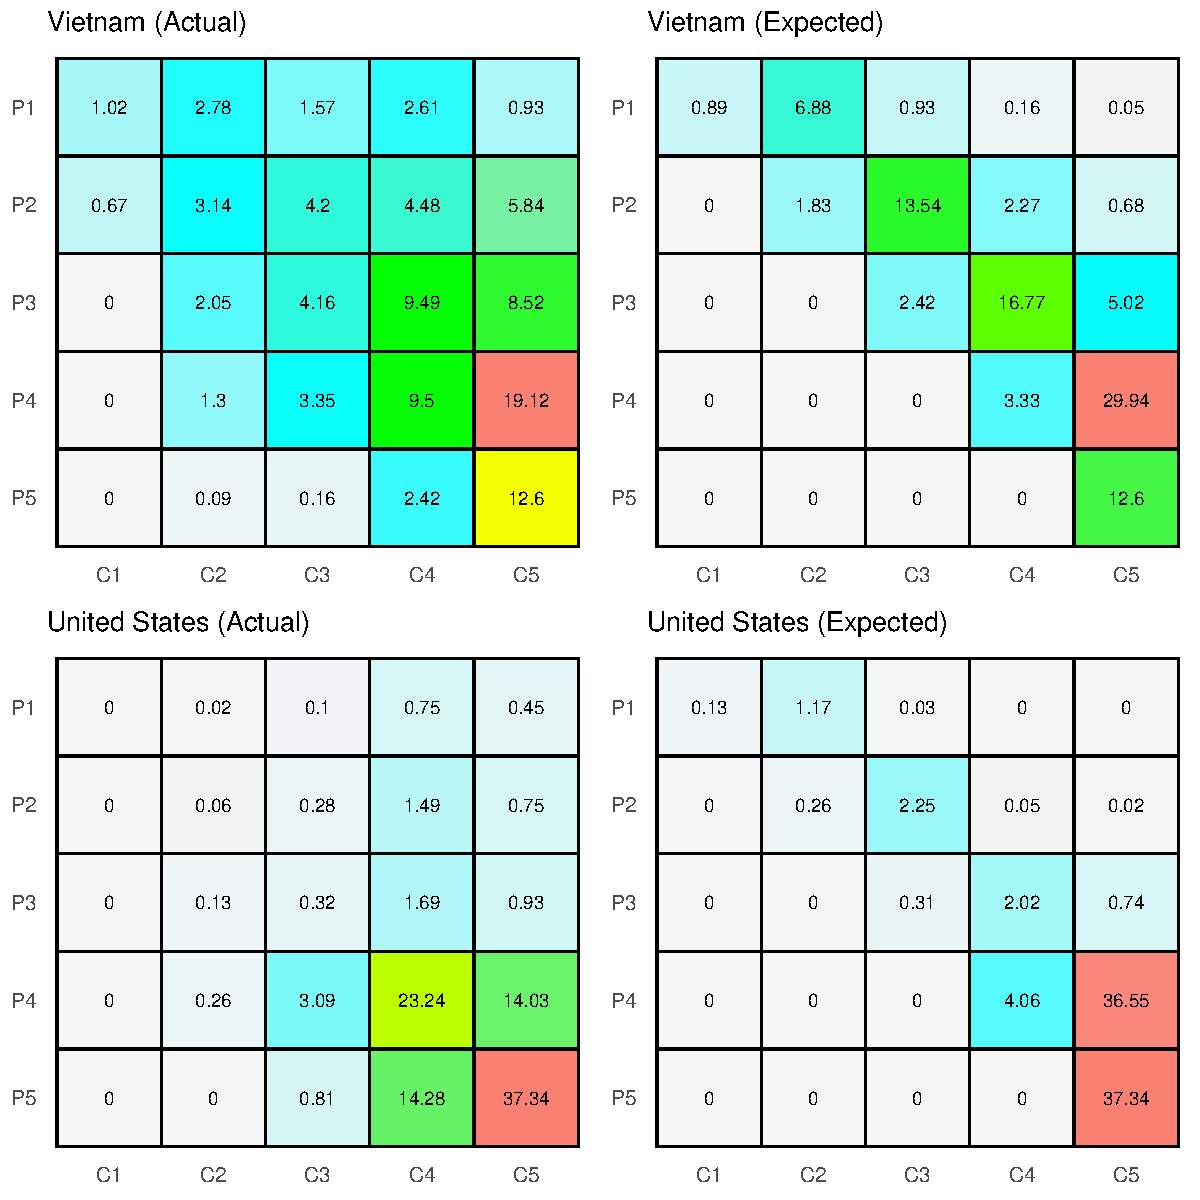
\includegraphics{figs/VNM_USA.pdf}}
    \caption{The expected matrices for Vietnam and The US}
    \label{fig:VNM_USA}
\end{figure}



\paragraph{The progress gap}

To calculate the progress gap between the actual $Q(x)$ and expected $P(x)$ matrices, f-divergences are utilized, which commonly include KL-divergence \citep{csiszar1975divergence}, Hellinger distance \citep{jeffreys1946invariant}, and total variation distance \citep{chatterjee2008distances}. The \textit{KL-divergence} is defined as

\[
D_{\text{KL}} = \sum_{x} P(x) \log \left[ \frac{P(x)}{Q(x)} \right].
\]
However, because \( P(x) \) and \( Q(x) \) can be zero or approaching zero, the KL-divergence can yield extremely high values, which may not always be desirable. In contrast, the \textit{Hellinger distance} provides a more robust measure, defined as

\[
\begin{aligned}
D_{\text{HL}} &= \frac{1}{\sqrt{2}} \sqrt{\sum_{x} \left( \sqrt{P(x)} - \sqrt{Q(x)} \right)^2} \\
&= \sqrt{\frac{1}{2} \sum_{x} \left[ \sqrt{P(x)} - \sqrt{Q(x)} \right]^2}
\end{aligned}.
\]
This formulation captures the differences between distributions without the issues associated with zero probabilities. Finally, the total variation distance is given by

\[
\begin{aligned}
D_{\text{TV}} &= \frac{1}{2} \sum_{x} |P(x) - Q(x)| \\
&= \frac{1}{2} \sum_{x} \left| \left[ \sqrt{P(x)} - \sqrt{Q(x)} \right] \left[ \sqrt{P(x)} + \sqrt{Q(x)} \right] \right|
\end{aligned}.
\]
While \textit{total variation distance} is another common measure, it is affected by the term \(\left[ \sqrt{P(x)} + \sqrt{Q(x)} \right]\), making it less sensitive to small differences compared to the Hellinger distance. As a result, the Hellinger distance is considered a more effective way to capture the gap between the actual and expected distributions.

Based on the Hellinger distance, we develop \textit{the Progress Gap} as a measure of social progress to calculate the distance between the actual matrix and the expected matrix. The Progress Gap \( D_{\text{PG}} \) is defined as:

\[
D_{\text{PG}} = \frac{1}{\sqrt{2}} \sum_{x \in U} \left[ \sqrt{P(x)} - \sqrt{Q(x)} \right] - \frac{1}{\sqrt{2}} \sum_{x \notin U} \left[ \sqrt{P(x)} - \sqrt{Q(x)} \right],
\]
where \( U \) is the set of probabilities in the upward area, defined as \( U = \{ (c,p) \mid 1 \leq c < p \leq 5 \} \cup \{ (5,5) \} \), with \( c \) representing the child’s education level and \( p \) representing the maximum parent’s education level. Unlike the Hellinger distance, which uses the absolute value \( \sqrt{[f(x)]^2} \) to measure the distance, we adjust the signs to fit the definition of social progress. Specifically, downward and persistent mobility are considered "bad" signs, while upward mobility is seen as a "good" sign. Since the expected value can be exceeded if a country implements effective radical education policies, resulting in \( \left[\sqrt{P(x)} - \sqrt{Q(x)}\right] < 0 \), this exceptional achievement is deducted from the progress gap, making the gap smaller. Because our progress gap index can be negative, exceeding the range of [0,1], we apply a max-min normalization to facilitate comparisons with both absolute and relative mobility:

\[
D_{\text{PG}|\text{norm}} = \frac{D_{\text{PG}} - \min(D_{\text{PG}})}{\max(D_{\text{PG}}) - \min(D_{\text{PG}})}.
\]

Since the goal of this research is to compare social progress among countries, normalization makes sense as it provides a relative measure rather than an absolute one, which is more sensitive to predefined assumptions. To ensure robustness, our methods should be applied consistently across countries using the same settings. This includes analyzing the same cohorts and employing the same comparison methods. Specifically, we recommend using the maximum education level of both parents versus the education level of the child, which has been considered the most reliable approach \citep{van2024intergenerational}. By maintaining these consistent criteria across different countries, we can better ensure that the progress gap measurement reflects meaningful and comparable social progress, minimizing potential biases that could arise from differing methods or population characteristics. This consistency is crucial for drawing valid comparisons and understanding social mobility across countries.

\section{Application to a new global dataset} \label{sec:application}


We apply our method to the Global Database on Intergenerational Mobility (GDIM), which consolidates data from over 400 household surveys, providing a comprehensive analysis of social mobility in education across 153 countries, representing about 97 percent of the global population, with the latest cohort from the 1980s. The unit of analysis represents each survey, including details such as the country, cohorts of respondents, survey year, methods for calculating parents' education (Mother/Father/Average/Max), methods for calculating children's education (Sons/Daughters/All), the number of observations, and key indicators such as the share of parents with different education levels, the share of children with different education levels, and measures of social mobility for that survey. Each survey has many metrics, including but not limited to: \textit{CAT}, which measures the probability that a child surpasses the parent’s educational category (conditional on the parent not having tertiary education); \textit{MIX}, which measures the probability of a child surpassing the parent’s educational category while considering children with tertiary education as mobile; \textit{CAT\_ISCED0} (equivalent to \textit{AHMP}), which tracks the probability of a child surpassing the parent’s educational category when parents have less than primary education; $COR$, the correlation coefficient between the children's and parents' years of schooling; \textit{BETA}, the beta coefficient from regressing children's years of schooling on parents' years of schooling; \textit{MU050}, the expected educational rank of a child born in the bottom half; \textit{BHQ4}, the probability that a child from the bottom half reaches the top quartile; and the Transition Matrix.

This study focuses on evaluating absolute mobility, measured by \textit{CAT}, and relative mobility, measured by 1-BETA. While local measures such as \textit{AHMP}, \textit{MU050}, and \textit{BHQ4} can be useful for assessing inequality among disadvantaged groups, they do not adequately capture social mobility at the societal level. Regarding absolute mobility, \textit{CAT} is more closely aligned with our index than \textit{MIX}. Although both measure upward mobility, they differ in how they account for the ceiling effect. \textit{CAT} ignores the ceiling effect by treating it as a form of intergenerational persistence, whereas MIX considers it a type of upward mobility. In our approach, the ceiling effect is viewed as both persistent and upward. Specifically, in the expected matrix, the probability that a child of the highest-educated parents attains the highest education level remains stable across generations, with the conditional probability always equal to 1, but stability is maintained only between parents and children due to the inflow of social mobility in subsequent generations. However, upward mobility is still present because, for other lower education levels, only 10\% of individuals should retain their parents' education level, implying that 90\% should experience upward mobility. In cases of ceiling upward mobility, individuals reach the highest education level, just like their parents. For relative mobility, we agree with \citet{van2024intergenerational} that \textit{1-BETA} better represents relative mobility compared to \textit{1-COR}, as \textit{BETA} is not influenced by education inequality in the child generation $\operatorname{Var}(Y_c)$. In summary, this study will compare different measures of social mobility, focusing on CAT, 1-BETA, and our proposed index.

\begin{figure}[H]
    \centering
    \scalebox{0.5}{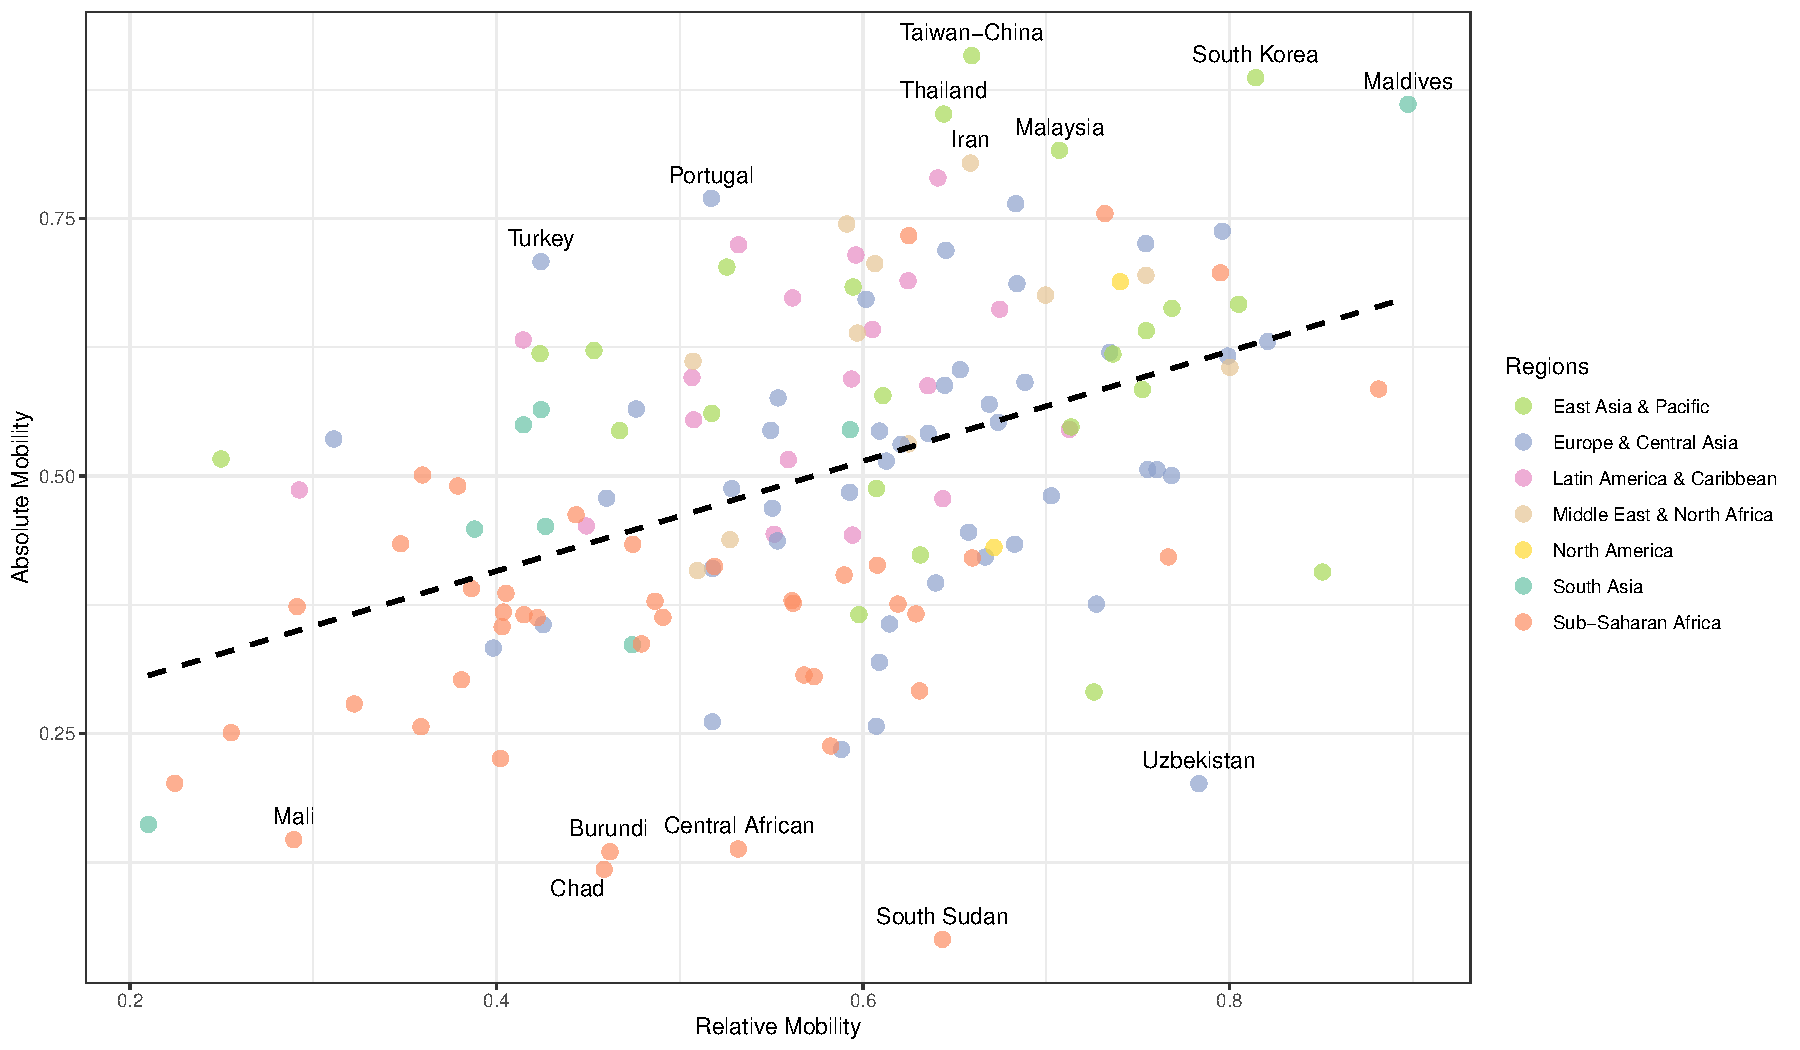
\includegraphics{figs/abs_rel.pdf}}
    \caption{Absolute and Relative Mobility}
    \label{fig:abs_rel}
\end{figure}

To compare with the mobility indexes reported in the World Bank's analysis using GDIM, the data is filtered by selecting parents' education as the maximum level (the most robust measure), children's education as all (gender-neutral), and the 1980s cohort (the latest available). Absolute and relative mobility in GDIM are presented in Figure \ref{fig:abs_rel}. There is a significant gap in interpretation between absolute mobility (\textit{CAT}, which captures upward trends) and relative mobility (\textit{1-BETA}, which reflects social fluidity). For example, in the case of South Sudan, relative mobility is relatively high, comparable to upper-middle-income countries like Thailand and Malaysia. However, South Sudan has the lowest absolute mobility, whereas Thailand and Malaysia rank among the highest in absolute mobility. While \citet{van2024intergenerational} "refrain from using the terms absolute and relative," treating them interchangeably under the single term "social mobility" should be reconsidered. Measures of absolute mobility, such as \textit{CAT} and \textit{MIX}, are often categorized as social mobility, but in reality, they assess social progress (albeit imperfectly) with a focus on upward trends. In contrast, measures of relative mobility, such as \textit{1-COR} and \textit{1-BETA}, are also framed as social mobility, but they actually capture social fluidity, which aligns more closely with concepts like entropy. While both social progress and social fluidity can be interpreted in terms of equality of opportunity, social progress is inherently directional.

\paragraph{New global rankings}

From GDIM, we calculate the progress gap as outlined in Section 3. The data cleaning process ensures that each transition matrix sums to 1, as the original GDIM data is set such that the total share of all children with the same family background equals 1, \(\sum_{i=1}^{5} \operatorname{Pr}[R_c = i| R_p] = 1\). Figure \ref{fig:rank} visually ranks countries based on our progress gap index and groups them into three equal-sized categories. Each bar represents a country, colored according to its region, allowing for regional comparisons of progress. The chart also includes three key mobility measures represented by different symbols: absolute mobility \textit{CAT} (blue squares), relative mobility \textit{1-BETA} (red circles), and a progressive measure \textit{MIX} (green triangles). The full details are shown in the  \ref{app:list}. According to our progress gap index, South Korea and Taiwan are the most progressive economies, linked to their exceptional economic development \citep{morris1996asia}, while the Central African Republic and Zambia rank the lowest. To provide a clearer regional distribution, we present the progress gap index on a global map. The results indicate that Africa and South Asia are less progressive, whereas most developed countries show higher progressiveness. Interestingly, Latin America demonstrates progress in education, but this does not translate into economic development. This can be explained by the mismatch between education and labor market outcomes in the region, as discussed by \citet{bassi2012disconnected}.

\begin{landscape}
\begin{figure}[H]
    \centering
    \scalebox{0.49}{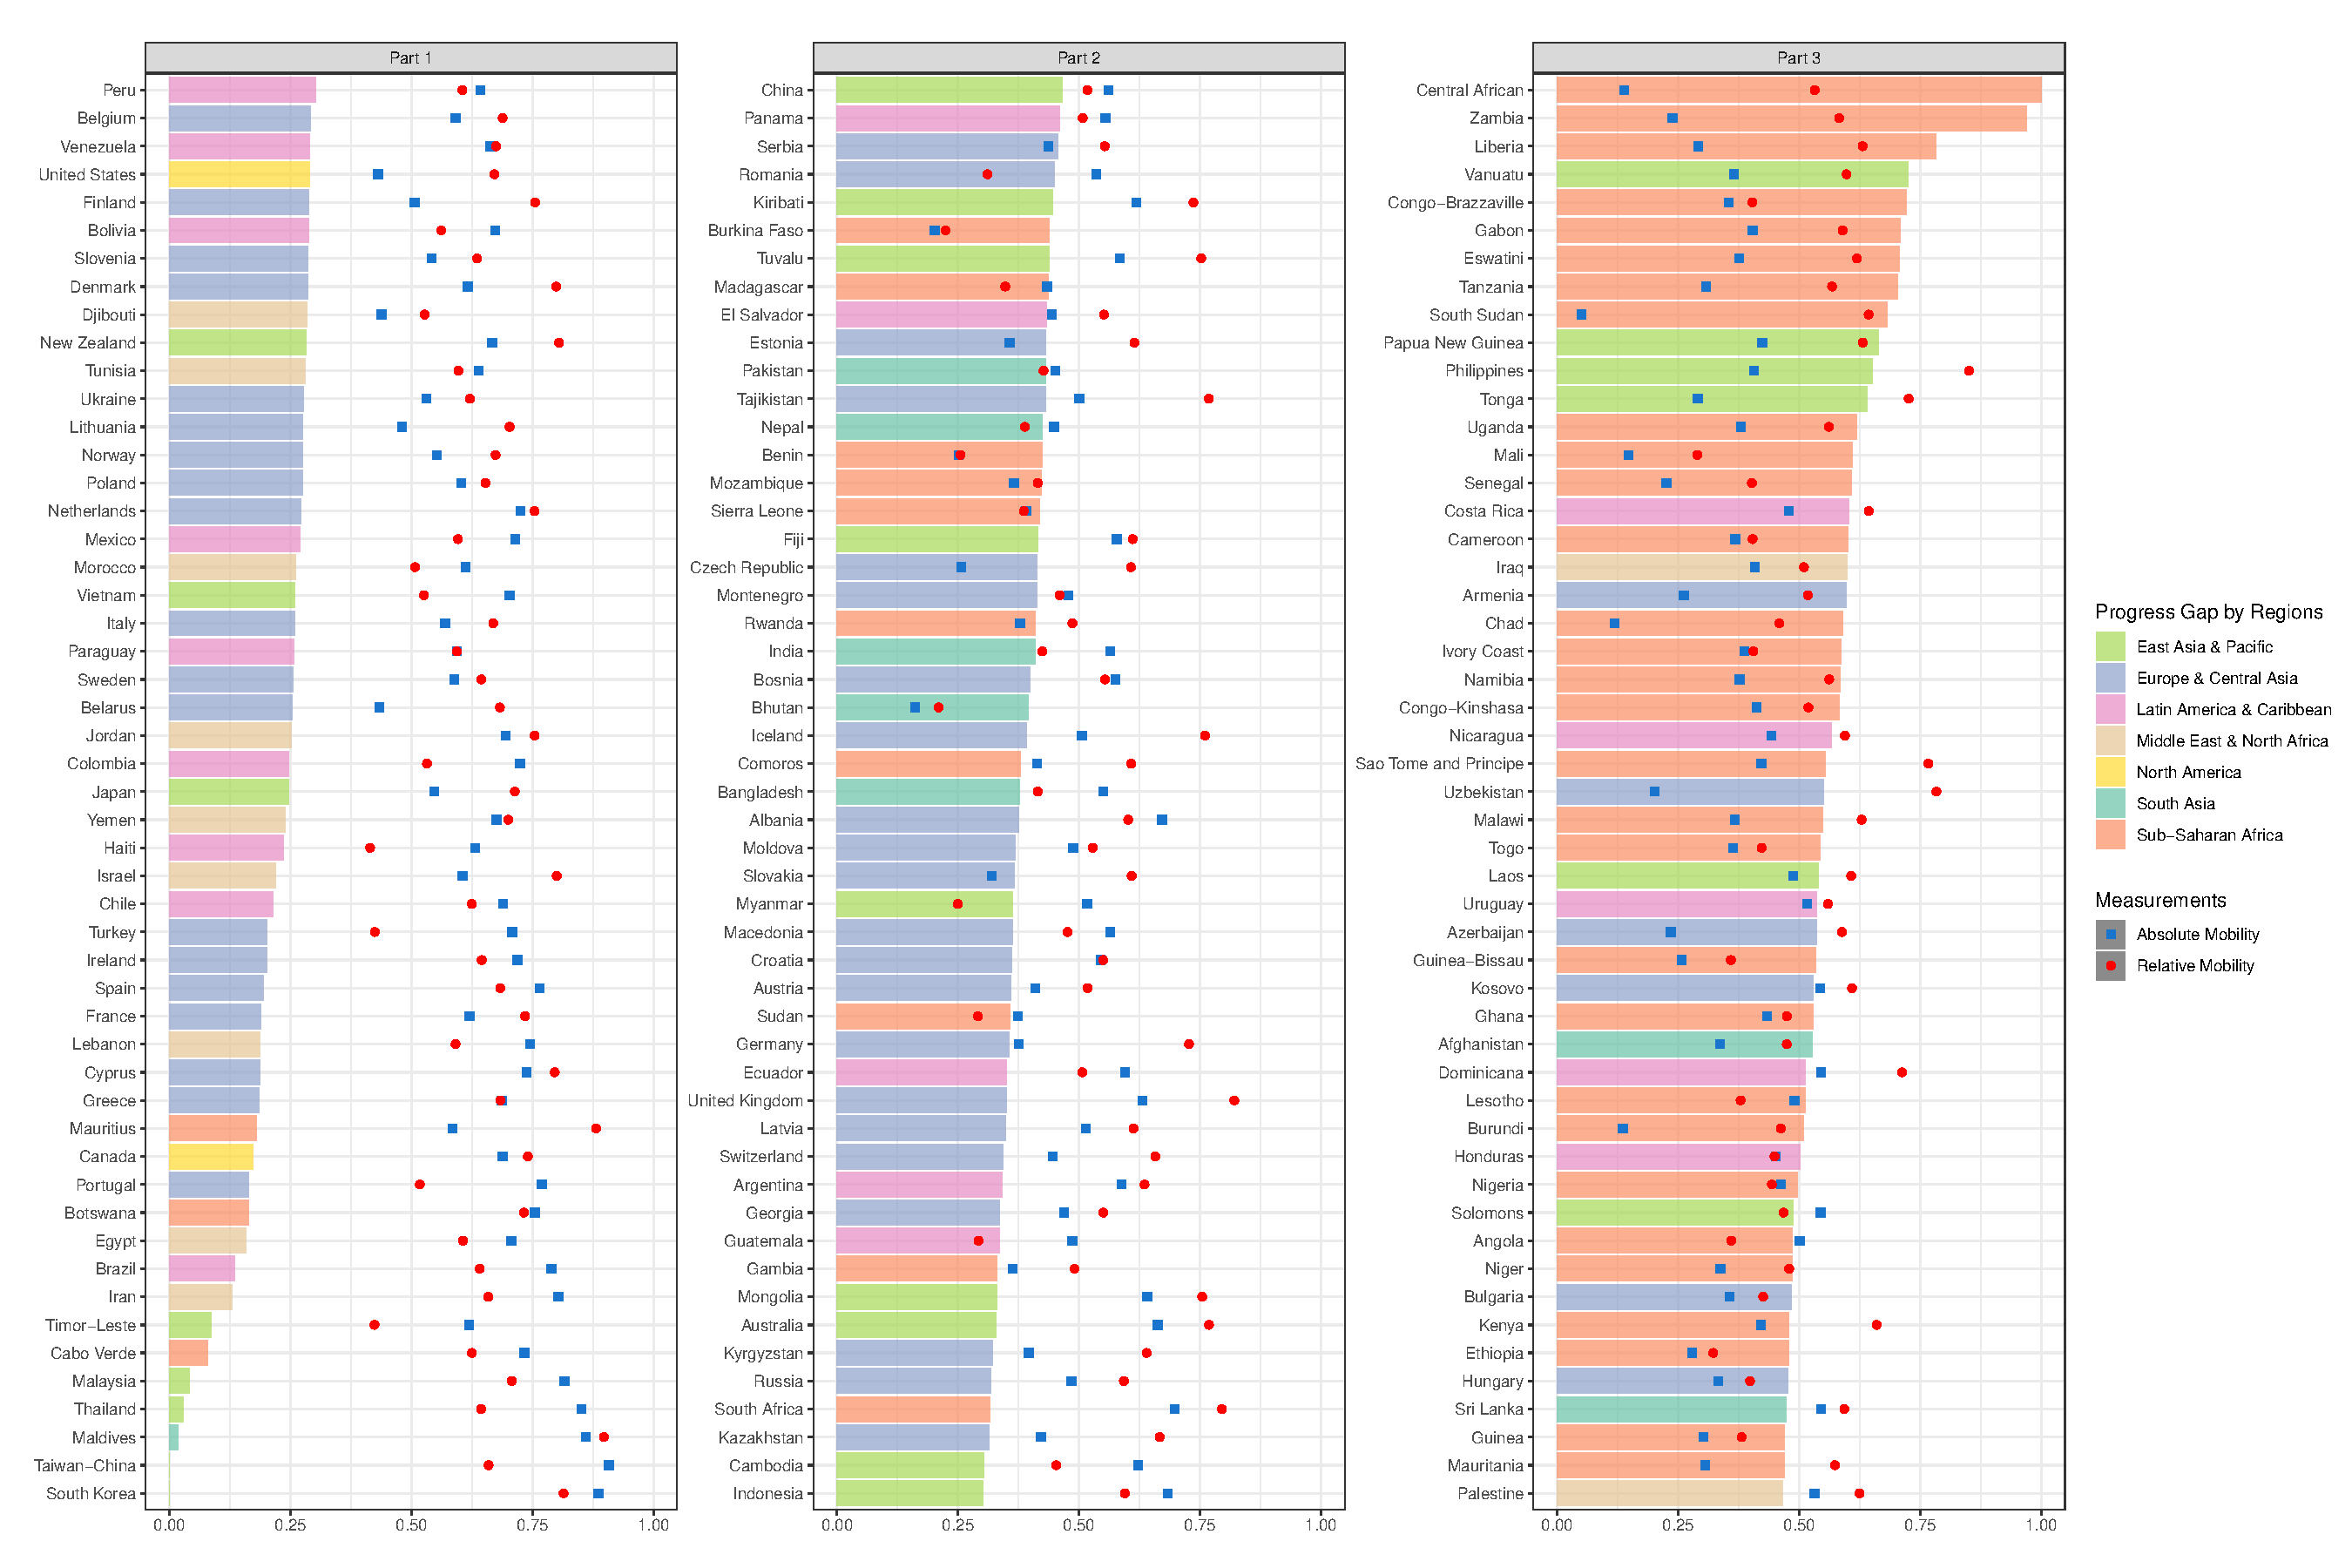
\includegraphics{figs/rank.pdf}}
    \caption{Global Rankings by Progress Gap}
    \label{fig:rank}
\end{figure}
\end{landscape} 

\begin{figure}[H]
    \centering
    \scalebox{0.55}{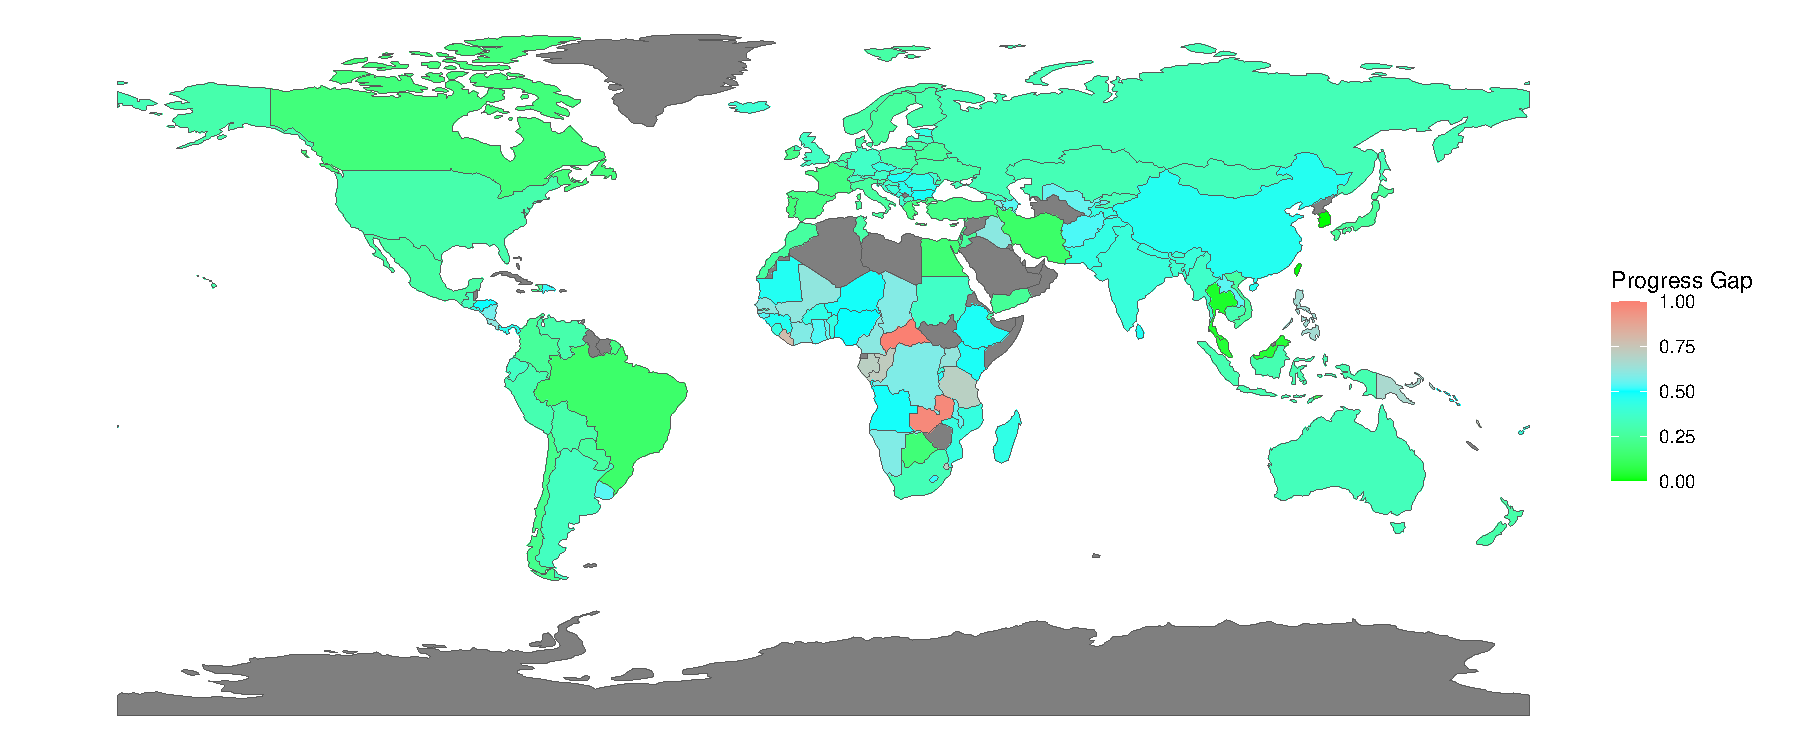
\includegraphics{figs/map.pdf}}
    \caption{Global mobility by a new measurement}
    \label{fig:map}
\end{figure}

One of the potentially controversial cases in our proposed index is Bhutan and Iceland, which appear next to each other in the ranking of the progress gap. To clarify this, we present their transition matrices in Figure \ref{fig:compare3}. It is evident that Bhutan lags significantly behind Iceland in both absolute mobility (0.16 vs. 0.51) and relative mobility (0.21 vs. 0.76). Additionally, Iceland's education distribution is far better than Bhutan’s, as most of Iceland’s population is highly educated, whereas the majority of Bhutan’s population has not attained even primary education. There is ample evidence to conclude that Iceland is much more progressive than Bhutan. However, this overlooks the difficulty problem when discussing equality of opportunity. Iceland’s initial conditions were significantly better than Bhutan’s, so a simple comparison based on education distribution alone is insufficient. Our measure, as the name implies, assesses the progress gap by evaluating the shortfall from the predefined target rather than the current status.  This case also illustrates a fundamental conflict between the concepts of social progress and social fluidity when both are used to assess equality of opportunity. Specifically, while we do not deny that Iceland likely provides greater social fluidity than Bhutan (as reflected in higher relative mobility), such freedom does not necessarily translate into social progress. As Figure \ref{fig:compare3} shows, Iceland’s downward mobility rate is just as high as its upward mobility rate. In summary, in terms of social progress, Bhutan and Iceland are nearly identical, despite their significant differences in social fluidity.


\begin{figure}[H]
    \centering
    \scalebox{0.55}{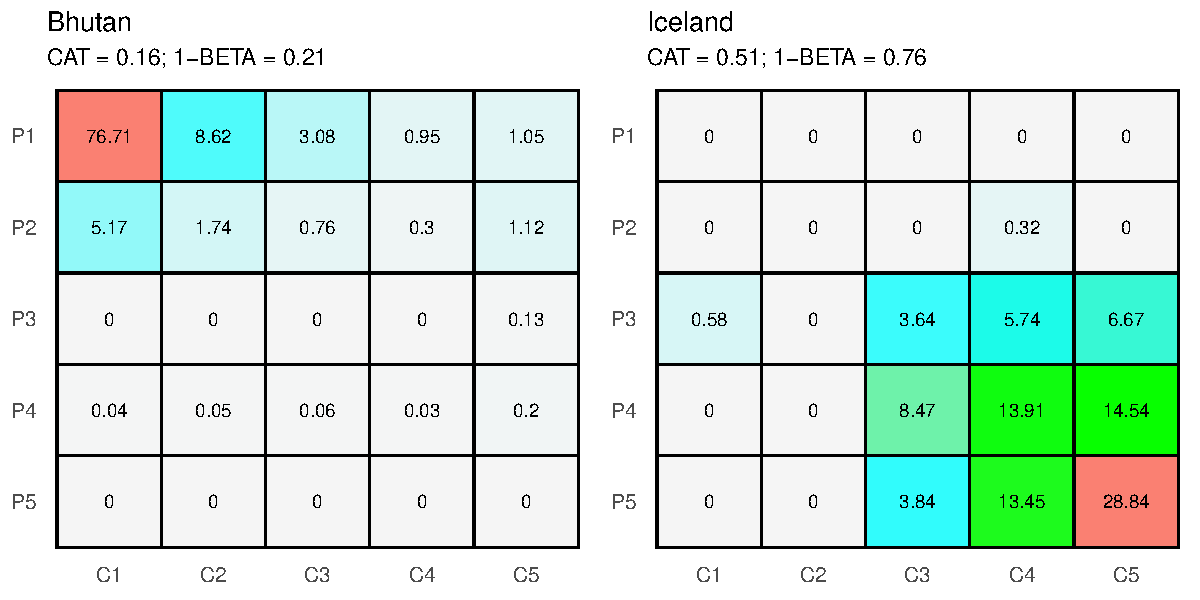
\includegraphics{figs/compare3.pdf}}
    \caption{Bhutan vs. Iceland}
    \label{fig:compare3}
    \captionsetup{font=footnotesize}
    \caption*{\textbf{Notes:} \textit{CAT} measures absolute mobility, \textit{1-BETA} measures relative mobility. The data is sourced from the Global Database on Intergenerational Mobility (2023). The analysis focuses on the 1980 cohort, comparing the education levels of all children to the maximum education level of their parents.}
\end{figure}

\paragraph{Comparison to current measures}
Finally, we examine the relationship between our new index, absolute mobility, and relative mobility using linear relationships in Figures \ref{fig:abs_pro} and \ref{fig:rel_pro}. Our index closely aligns with absolute mobility in capturing social progress and shows minimal outliers. However, while both measure social progress, our index is more advanced as it addresses the directionality problem. Due to this limitation, absolute mobility fails to differentiate between countries experiencing a downward trend, such as the Central African Republic and Zambia, and those with more persistent trends, such as Burundi, Bhutan, and Burkina Faso. Compared to relative mobility, our index highlights significant differences stemming from the fundamental distinction between social fluidity and social progress, as discussed earlier. For instance, both Timor-Leste (Figure \ref{fig:compare1}) and the Central African Republic (Figure \ref{fig:compare2}) exhibit high relative mobility. However, Timor-Leste’s mobility is upward, whereas the Central African Republic’s is downward. Regarding the difficulty problem, Figures \ref{fig:compare2} (current measures) and \ref{fig:rank} (our index) illustrate the case of Canada and Timor-Leste. Under our framework, Timor-Leste appears more progressive than Canada because it has had greater success in achieving efforts toward social progress, even though Canada has a much higher level of education. In this case, we also account for the ceiling effect. In summary, our index provides a more robust measure of social mobility than existing metrics.

\begin{figure}[H]
    \centering
    \scalebox{0.5}{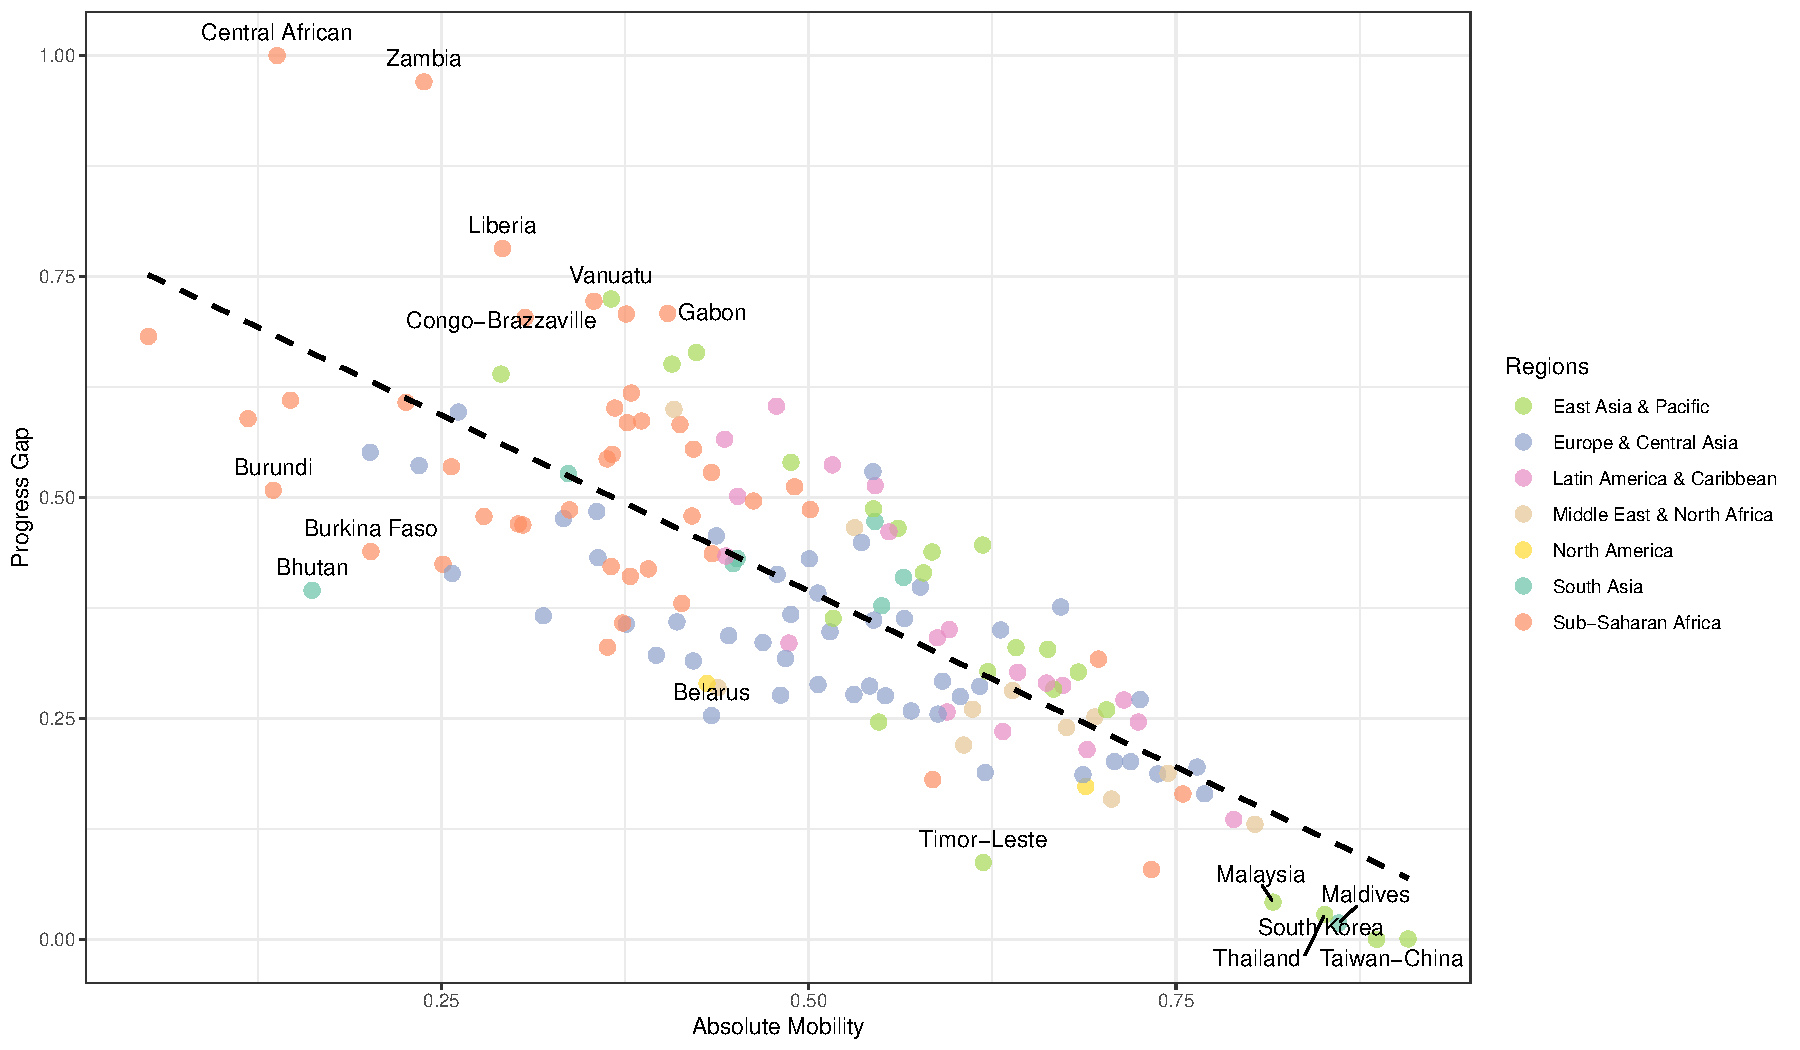
\includegraphics{figs/abs_pro.pdf}}
    \caption{Compared to absolute mobility}
    \label{fig:abs_pro}
\end{figure}

\begin{figure}[H]
    \centering
    \scalebox{0.5}{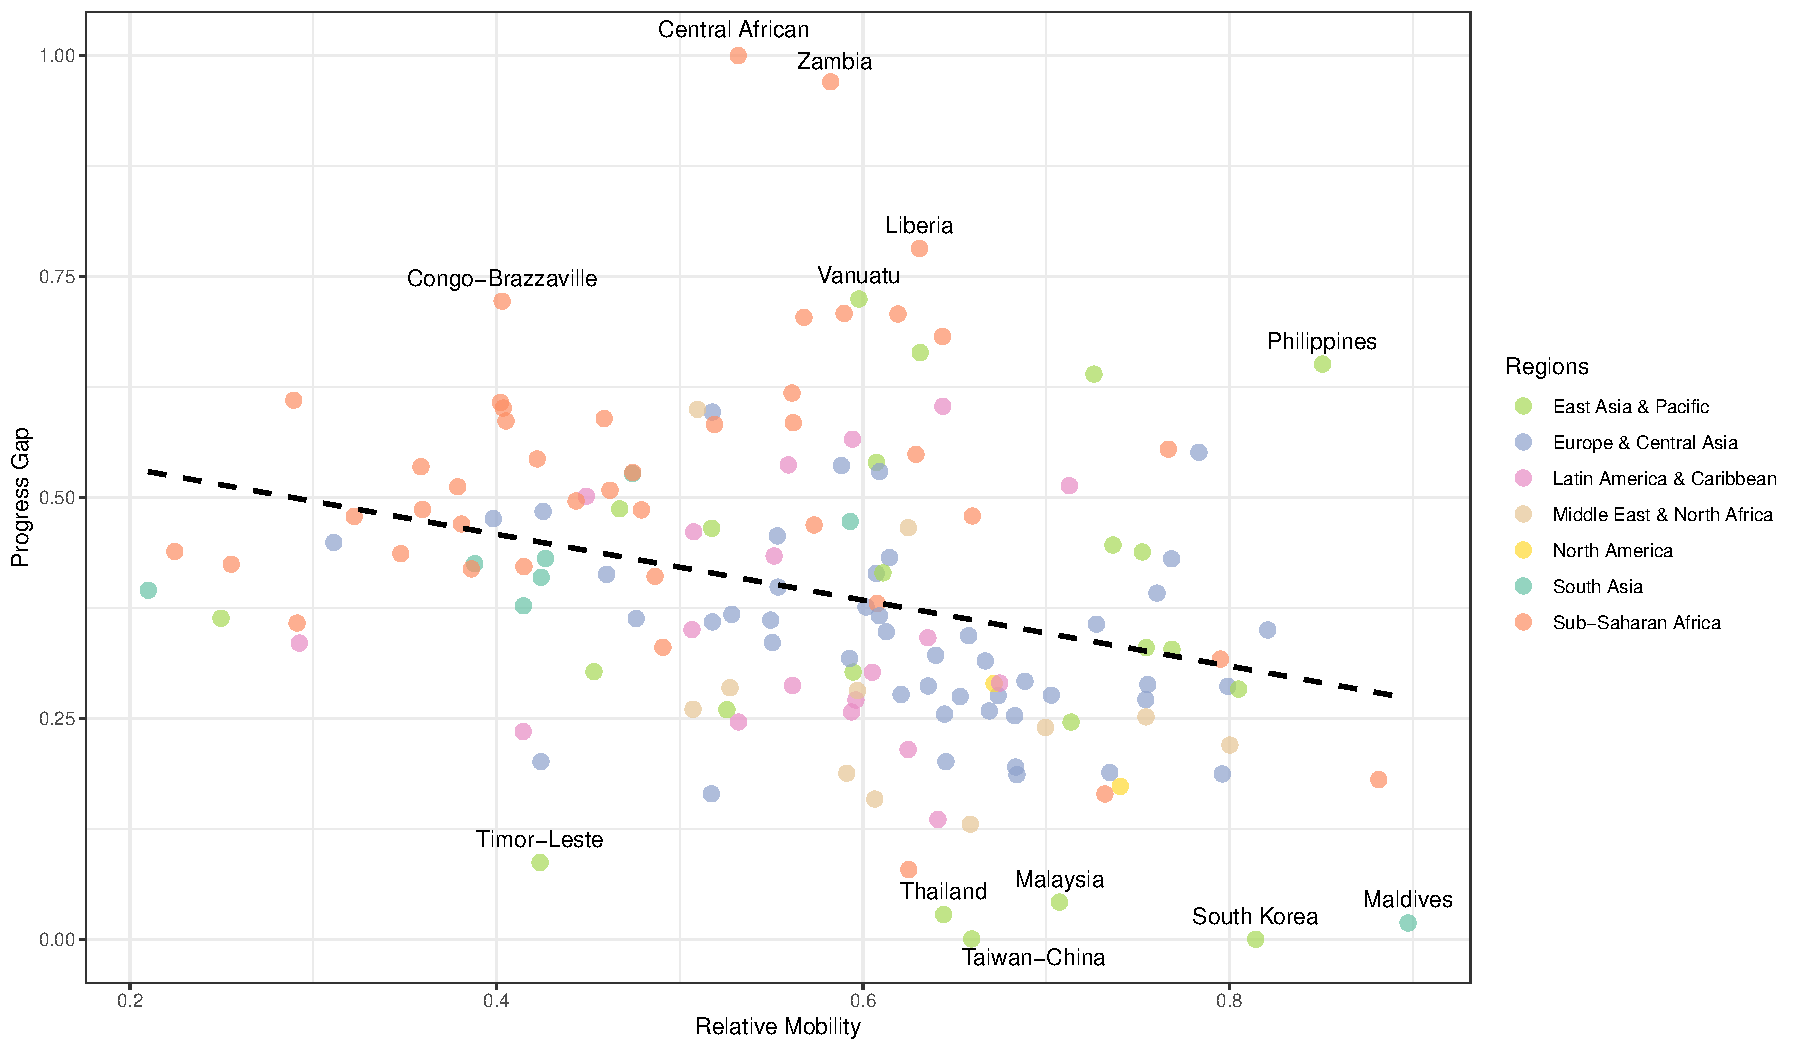
\includegraphics{figs/rel_pro.pdf}}
    \caption{Compared to relative mobility}
    \label{fig:rel_pro}
\end{figure}


\section{Conclusion} \label{sec:conclusion}

Current measures of social mobility fail to fully capture social progress in education. For example, although Bhutan and the Central African Republic exhibit comparable absolute mobility levels, the greater relative mobility in the Central African Republic stems from more frequent downward mobility, which does not indicate actual progress. Similarly, although Canada and Timor-Leste exhibit different mobility levels, the effort required for mobility in Timor-Leste is much greater, suggesting a different form of progress. To address these issues, this study develops a new index based on transition matrices, offering a more rigorous measure of educational social progress. By constructing an expected transition matrix that accounts for country-specific factors, this approach isolates genuine progress while filtering out persistent institutional and cultural constraints. The resulting measure aligns countries to a common reference frame, allowing for more meaningful comparisons of national efforts to advance social mobility through education. Our progress gap index, calculated using data from the GDIM, provides a clearer assessment. It shows that South Korea and Taiwan are the most progressive in terms of educational mobility, while countries like the Central African Republic and Zambia rank the lowest. Regional trends reveal that Africa and South Asia are less progressive, while most developed countries show higher progress.

Although our method is based on the World Bank’s approach and reports, the scope of this study extends beyond the confines of this study. The current measures we review are not exclusive to the World Bank; they are widely used in the field of social mobility \citep{corak2020canadian, chetty2014land, asher2019getting, alesina2021intergenerational, chetty2017fading}. To clarify, we are not studying a unique measurement used by one organization for its own report, but rather evaluating common measures in the field that have been compiled and applied by the World Bank in its recent database release. Moreover, our method can be extended to other ordinal measurements using mobility tables, such as self-reported health \citep{halliday2021intergenerational} or well-being \citep{molina2011intergenerational}. However, this would require further research and testing. One limitation of our method is its sensitivity to the selection of the true effect of intergenerational transmission, as some studies may report the effect as slightly larger - that is $\omega=0.15$, as shown by \citet{fleury2018intergenerational}. Nonetheless, this does not significantly change the overall findings of our study (see \ref{app:sensitive}).

\section*{Supplementary material}
An online appendix for this article is available on the journal's website.

\section*{Data availability}
The data and code supporting the findings of this study are available at \url{https://github.com/duongkhanhk29/MEASURE_MOBILITY/}.

\bibliographystyle{elsarticle-harv}
\bibliography{03_ref}


\appendix

\newpage
\section{List of countries} \label{app:list}

\tiny
\begin{longtblr}[
  label = none,
  entry = none,
]{
  width = \linewidth,
  colspec = {Q[54]Q[250]Q[280]Q[80]Q[100]Q[120]Q[100]Q[100]},
  row{1} = {c},
  cell{2}{1} = {c},
  cell{2}{4} = {c},
  cell{2}{5} = {c},
  cell{2}{6} = {c},
  cell{2}{7} = {c},
  cell{2}{8} = {c},
  cell{3}{1} = {c},
  cell{3}{4} = {c},
  cell{3}{5} = {c},
  cell{3}{6} = {c},
  cell{3}{7} = {c},
  cell{3}{8} = {c},
  cell{4}{1} = {c},
  cell{4}{4} = {c},
  cell{4}{5} = {c},
  cell{4}{6} = {c},
  cell{4}{7} = {c},
  cell{4}{8} = {c},
  cell{5}{1} = {c},
  cell{5}{4} = {c},
  cell{5}{5} = {c},
  cell{5}{6} = {c},
  cell{5}{7} = {c},
  cell{5}{8} = {c},
  cell{6}{1} = {c},
  cell{6}{4} = {c},
  cell{6}{5} = {c},
  cell{6}{6} = {c},
  cell{6}{7} = {c},
  cell{6}{8} = {c},
  cell{7}{1} = {c},
  cell{7}{4} = {c},
  cell{7}{5} = {c},
  cell{7}{6} = {c},
  cell{7}{7} = {c},
  cell{7}{8} = {c},
  cell{8}{1} = {c},
  cell{8}{4} = {c},
  cell{8}{5} = {c},
  cell{8}{6} = {c},
  cell{8}{7} = {c},
  cell{8}{8} = {c},
  cell{9}{1} = {c},
  cell{9}{4} = {c},
  cell{9}{5} = {c},
  cell{9}{6} = {c},
  cell{9}{7} = {c},
  cell{9}{8} = {c},
  cell{10}{1} = {c},
  cell{10}{4} = {c},
  cell{10}{5} = {c},
  cell{10}{6} = {c},
  cell{10}{7} = {c},
  cell{10}{8} = {c},
  cell{11}{1} = {c},
  cell{11}{4} = {c},
  cell{11}{5} = {c},
  cell{11}{6} = {c},
  cell{11}{7} = {c},
  cell{11}{8} = {c},
  cell{12}{1} = {c},
  cell{12}{4} = {c},
  cell{12}{5} = {c},
  cell{12}{6} = {c},
  cell{12}{7} = {c},
  cell{12}{8} = {c},
  cell{13}{1} = {c},
  cell{13}{4} = {c},
  cell{13}{5} = {c},
  cell{13}{6} = {c},
  cell{13}{7} = {c},
  cell{13}{8} = {c},
  cell{14}{1} = {c},
  cell{14}{4} = {c},
  cell{14}{5} = {c},
  cell{14}{6} = {c},
  cell{14}{7} = {c},
  cell{14}{8} = {c},
  cell{15}{1} = {c},
  cell{15}{4} = {c},
  cell{15}{5} = {c},
  cell{15}{6} = {c},
  cell{15}{7} = {c},
  cell{15}{8} = {c},
  cell{16}{1} = {c},
  cell{16}{4} = {c},
  cell{16}{5} = {c},
  cell{16}{6} = {c},
  cell{16}{7} = {c},
  cell{16}{8} = {c},
  cell{17}{1} = {c},
  cell{17}{4} = {c},
  cell{17}{5} = {c},
  cell{17}{6} = {c},
  cell{17}{7} = {c},
  cell{17}{8} = {c},
  cell{18}{1} = {c},
  cell{18}{4} = {c},
  cell{18}{5} = {c},
  cell{18}{6} = {c},
  cell{18}{7} = {c},
  cell{18}{8} = {c},
  cell{19}{1} = {c},
  cell{19}{4} = {c},
  cell{19}{5} = {c},
  cell{19}{6} = {c},
  cell{19}{7} = {c},
  cell{19}{8} = {c},
  cell{20}{1} = {c},
  cell{20}{4} = {c},
  cell{20}{5} = {c},
  cell{20}{6} = {c},
  cell{20}{7} = {c},
  cell{20}{8} = {c},
  cell{21}{1} = {c},
  cell{21}{4} = {c},
  cell{21}{5} = {c},
  cell{21}{6} = {c},
  cell{21}{7} = {c},
  cell{21}{8} = {c},
  cell{22}{1} = {c},
  cell{22}{4} = {c},
  cell{22}{5} = {c},
  cell{22}{6} = {c},
  cell{22}{7} = {c},
  cell{22}{8} = {c},
  cell{23}{1} = {c},
  cell{23}{4} = {c},
  cell{23}{5} = {c},
  cell{23}{6} = {c},
  cell{23}{7} = {c},
  cell{23}{8} = {c},
  cell{24}{1} = {c},
  cell{24}{4} = {c},
  cell{24}{5} = {c},
  cell{24}{6} = {c},
  cell{24}{7} = {c},
  cell{24}{8} = {c},
  cell{25}{1} = {c},
  cell{25}{4} = {c},
  cell{25}{5} = {c},
  cell{25}{6} = {c},
  cell{25}{7} = {c},
  cell{25}{8} = {c},
  cell{26}{1} = {c},
  cell{26}{4} = {c},
  cell{26}{5} = {c},
  cell{26}{6} = {c},
  cell{26}{7} = {c},
  cell{26}{8} = {c},
  cell{27}{1} = {c},
  cell{27}{4} = {c},
  cell{27}{5} = {c},
  cell{27}{6} = {c},
  cell{27}{7} = {c},
  cell{27}{8} = {c},
  cell{28}{1} = {c},
  cell{28}{4} = {c},
  cell{28}{5} = {c},
  cell{28}{6} = {c},
  cell{28}{7} = {c},
  cell{28}{8} = {c},
  cell{29}{1} = {c},
  cell{29}{4} = {c},
  cell{29}{5} = {c},
  cell{29}{6} = {c},
  cell{29}{7} = {c},
  cell{29}{8} = {c},
  cell{30}{1} = {c},
  cell{30}{4} = {c},
  cell{30}{5} = {c},
  cell{30}{6} = {c},
  cell{30}{7} = {c},
  cell{30}{8} = {c},
  cell{31}{1} = {c},
  cell{31}{4} = {c},
  cell{31}{5} = {c},
  cell{31}{6} = {c},
  cell{31}{7} = {c},
  cell{31}{8} = {c},
  cell{32}{1} = {c},
  cell{32}{4} = {c},
  cell{32}{5} = {c},
  cell{32}{6} = {c},
  cell{32}{7} = {c},
  cell{32}{8} = {c},
  cell{33}{1} = {c},
  cell{33}{4} = {c},
  cell{33}{5} = {c},
  cell{33}{6} = {c},
  cell{33}{7} = {c},
  cell{33}{8} = {c},
  cell{34}{1} = {c},
  cell{34}{4} = {c},
  cell{34}{5} = {c},
  cell{34}{6} = {c},
  cell{34}{7} = {c},
  cell{34}{8} = {c},
  cell{35}{1} = {c},
  cell{35}{4} = {c},
  cell{35}{5} = {c},
  cell{35}{6} = {c},
  cell{35}{7} = {c},
  cell{35}{8} = {c},
  cell{36}{1} = {c},
  cell{36}{4} = {c},
  cell{36}{5} = {c},
  cell{36}{6} = {c},
  cell{36}{7} = {c},
  cell{36}{8} = {c},
  cell{37}{1} = {c},
  cell{37}{4} = {c},
  cell{37}{5} = {c},
  cell{37}{6} = {c},
  cell{37}{7} = {c},
  cell{37}{8} = {c},
  cell{38}{1} = {c},
  cell{38}{4} = {c},
  cell{38}{5} = {c},
  cell{38}{6} = {c},
  cell{38}{7} = {c},
  cell{38}{8} = {c},
  cell{39}{1} = {c},
  cell{39}{4} = {c},
  cell{39}{5} = {c},
  cell{39}{6} = {c},
  cell{39}{7} = {c},
  cell{39}{8} = {c},
  cell{40}{1} = {c},
  cell{40}{4} = {c},
  cell{40}{5} = {c},
  cell{40}{6} = {c},
  cell{40}{7} = {c},
  cell{40}{8} = {c},
  cell{41}{1} = {c},
  cell{41}{4} = {c},
  cell{41}{5} = {c},
  cell{41}{6} = {c},
  cell{41}{7} = {c},
  cell{41}{8} = {c},
  cell{42}{1} = {c},
  cell{42}{4} = {c},
  cell{42}{5} = {c},
  cell{42}{6} = {c},
  cell{42}{7} = {c},
  cell{42}{8} = {c},
  cell{43}{1} = {c},
  cell{43}{4} = {c},
  cell{43}{5} = {c},
  cell{43}{6} = {c},
  cell{43}{7} = {c},
  cell{43}{8} = {c},
  cell{44}{1} = {c},
  cell{44}{4} = {c},
  cell{44}{5} = {c},
  cell{44}{6} = {c},
  cell{44}{7} = {c},
  cell{44}{8} = {c},
  cell{45}{1} = {c},
  cell{45}{4} = {c},
  cell{45}{5} = {c},
  cell{45}{6} = {c},
  cell{45}{7} = {c},
  cell{45}{8} = {c},
  cell{46}{1} = {c},
  cell{46}{4} = {c},
  cell{46}{5} = {c},
  cell{46}{6} = {c},
  cell{46}{7} = {c},
  cell{46}{8} = {c},
  cell{47}{1} = {c},
  cell{47}{4} = {c},
  cell{47}{5} = {c},
  cell{47}{6} = {c},
  cell{47}{7} = {c},
  cell{47}{8} = {c},
  cell{48}{1} = {c},
  cell{48}{4} = {c},
  cell{48}{5} = {c},
  cell{48}{6} = {c},
  cell{48}{7} = {c},
  cell{48}{8} = {c},
  cell{49}{1} = {c},
  cell{49}{4} = {c},
  cell{49}{5} = {c},
  cell{49}{6} = {c},
  cell{49}{7} = {c},
  cell{49}{8} = {c},
  cell{50}{1} = {c},
  cell{50}{4} = {c},
  cell{50}{5} = {c},
  cell{50}{6} = {c},
  cell{50}{7} = {c},
  cell{50}{8} = {c},
  cell{51}{1} = {c},
  cell{51}{4} = {c},
  cell{51}{5} = {c},
  cell{51}{6} = {c},
  cell{51}{7} = {c},
  cell{51}{8} = {c},
  cell{52}{1} = {c},
  cell{52}{4} = {c},
  cell{52}{5} = {c},
  cell{52}{6} = {c},
  cell{52}{7} = {c},
  cell{52}{8} = {c},
  cell{53}{1} = {c},
  cell{53}{4} = {c},
  cell{53}{5} = {c},
  cell{53}{6} = {c},
  cell{53}{7} = {c},
  cell{53}{8} = {c},
  cell{54}{1} = {c},
  cell{54}{4} = {c},
  cell{54}{5} = {c},
  cell{54}{6} = {c},
  cell{54}{7} = {c},
  cell{54}{8} = {c},
  cell{55}{1} = {c},
  cell{55}{4} = {c},
  cell{55}{5} = {c},
  cell{55}{6} = {c},
  cell{55}{7} = {c},
  cell{55}{8} = {c},
  cell{56}{1} = {c},
  cell{56}{4} = {c},
  cell{56}{5} = {c},
  cell{56}{6} = {c},
  cell{56}{7} = {c},
  cell{56}{8} = {c},
  cell{57}{1} = {c},
  cell{57}{4} = {c},
  cell{57}{5} = {c},
  cell{57}{6} = {c},
  cell{57}{7} = {c},
  cell{57}{8} = {c},
  cell{58}{1} = {c},
  cell{58}{4} = {c},
  cell{58}{5} = {c},
  cell{58}{6} = {c},
  cell{58}{7} = {c},
  cell{58}{8} = {c},
  cell{59}{1} = {c},
  cell{59}{4} = {c},
  cell{59}{5} = {c},
  cell{59}{6} = {c},
  cell{59}{7} = {c},
  cell{59}{8} = {c},
  cell{60}{1} = {c},
  cell{60}{4} = {c},
  cell{60}{5} = {c},
  cell{60}{6} = {c},
  cell{60}{7} = {c},
  cell{60}{8} = {c},
  cell{61}{1} = {c},
  cell{61}{4} = {c},
  cell{61}{5} = {c},
  cell{61}{6} = {c},
  cell{61}{7} = {c},
  cell{61}{8} = {c},
  cell{62}{1} = {c},
  cell{62}{4} = {c},
  cell{62}{5} = {c},
  cell{62}{6} = {c},
  cell{62}{7} = {c},
  cell{62}{8} = {c},
  cell{63}{1} = {c},
  cell{63}{4} = {c},
  cell{63}{5} = {c},
  cell{63}{6} = {c},
  cell{63}{7} = {c},
  cell{63}{8} = {c},
  cell{64}{1} = {c},
  cell{64}{4} = {c},
  cell{64}{5} = {c},
  cell{64}{6} = {c},
  cell{64}{7} = {c},
  cell{64}{8} = {c},
  cell{65}{1} = {c},
  cell{65}{4} = {c},
  cell{65}{5} = {c},
  cell{65}{6} = {c},
  cell{65}{7} = {c},
  cell{65}{8} = {c},
  cell{66}{1} = {c},
  cell{66}{4} = {c},
  cell{66}{5} = {c},
  cell{66}{6} = {c},
  cell{66}{7} = {c},
  cell{66}{8} = {c},
  cell{67}{1} = {c},
  cell{67}{4} = {c},
  cell{67}{5} = {c},
  cell{67}{6} = {c},
  cell{67}{7} = {c},
  cell{67}{8} = {c},
  cell{68}{1} = {c},
  cell{68}{4} = {c},
  cell{68}{5} = {c},
  cell{68}{6} = {c},
  cell{68}{7} = {c},
  cell{68}{8} = {c},
  cell{69}{1} = {c},
  cell{69}{4} = {c},
  cell{69}{5} = {c},
  cell{69}{6} = {c},
  cell{69}{7} = {c},
  cell{69}{8} = {c},
  cell{70}{1} = {c},
  cell{70}{4} = {c},
  cell{70}{5} = {c},
  cell{70}{6} = {c},
  cell{70}{7} = {c},
  cell{70}{8} = {c},
  cell{71}{1} = {c},
  cell{71}{4} = {c},
  cell{71}{5} = {c},
  cell{71}{6} = {c},
  cell{71}{7} = {c},
  cell{71}{8} = {c},
  cell{72}{1} = {c},
  cell{72}{4} = {c},
  cell{72}{5} = {c},
  cell{72}{6} = {c},
  cell{72}{7} = {c},
  cell{72}{8} = {c},
  cell{73}{1} = {c},
  cell{73}{4} = {c},
  cell{73}{5} = {c},
  cell{73}{6} = {c},
  cell{73}{7} = {c},
  cell{73}{8} = {c},
  cell{74}{1} = {c},
  cell{74}{4} = {c},
  cell{74}{5} = {c},
  cell{74}{6} = {c},
  cell{74}{7} = {c},
  cell{74}{8} = {c},
  cell{75}{1} = {c},
  cell{75}{4} = {c},
  cell{75}{5} = {c},
  cell{75}{6} = {c},
  cell{75}{7} = {c},
  cell{75}{8} = {c},
  cell{76}{1} = {c},
  cell{76}{4} = {c},
  cell{76}{5} = {c},
  cell{76}{6} = {c},
  cell{76}{7} = {c},
  cell{76}{8} = {c},
  cell{77}{1} = {c},
  cell{77}{4} = {c},
  cell{77}{5} = {c},
  cell{77}{6} = {c},
  cell{77}{7} = {c},
  cell{77}{8} = {c},
  cell{78}{1} = {c},
  cell{78}{4} = {c},
  cell{78}{5} = {c},
  cell{78}{6} = {c},
  cell{78}{7} = {c},
  cell{78}{8} = {c},
  cell{79}{1} = {c},
  cell{79}{4} = {c},
  cell{79}{5} = {c},
  cell{79}{6} = {c},
  cell{79}{7} = {c},
  cell{79}{8} = {c},
  cell{80}{1} = {c},
  cell{80}{4} = {c},
  cell{80}{5} = {c},
  cell{80}{6} = {c},
  cell{80}{7} = {c},
  cell{80}{8} = {c},
  cell{81}{1} = {c},
  cell{81}{4} = {c},
  cell{81}{5} = {c},
  cell{81}{6} = {c},
  cell{81}{7} = {c},
  cell{81}{8} = {c},
  cell{82}{1} = {c},
  cell{82}{4} = {c},
  cell{82}{5} = {c},
  cell{82}{6} = {c},
  cell{82}{7} = {c},
  cell{82}{8} = {c},
  cell{83}{1} = {c},
  cell{83}{4} = {c},
  cell{83}{5} = {c},
  cell{83}{6} = {c},
  cell{83}{7} = {c},
  cell{83}{8} = {c},
  cell{84}{1} = {c},
  cell{84}{4} = {c},
  cell{84}{5} = {c},
  cell{84}{6} = {c},
  cell{84}{7} = {c},
  cell{84}{8} = {c},
  cell{85}{1} = {c},
  cell{85}{4} = {c},
  cell{85}{5} = {c},
  cell{85}{6} = {c},
  cell{85}{7} = {c},
  cell{85}{8} = {c},
  cell{86}{1} = {c},
  cell{86}{4} = {c},
  cell{86}{5} = {c},
  cell{86}{6} = {c},
  cell{86}{7} = {c},
  cell{86}{8} = {c},
  cell{87}{1} = {c},
  cell{87}{4} = {c},
  cell{87}{5} = {c},
  cell{87}{6} = {c},
  cell{87}{7} = {c},
  cell{87}{8} = {c},
  cell{88}{1} = {c},
  cell{88}{4} = {c},
  cell{88}{5} = {c},
  cell{88}{6} = {c},
  cell{88}{7} = {c},
  cell{88}{8} = {c},
  cell{89}{1} = {c},
  cell{89}{4} = {c},
  cell{89}{5} = {c},
  cell{89}{6} = {c},
  cell{89}{7} = {c},
  cell{89}{8} = {c},
  cell{90}{1} = {c},
  cell{90}{4} = {c},
  cell{90}{5} = {c},
  cell{90}{6} = {c},
  cell{90}{7} = {c},
  cell{90}{8} = {c},
  cell{91}{1} = {c},
  cell{91}{4} = {c},
  cell{91}{5} = {c},
  cell{91}{6} = {c},
  cell{91}{7} = {c},
  cell{91}{8} = {c},
  cell{92}{1} = {c},
  cell{92}{4} = {c},
  cell{92}{5} = {c},
  cell{92}{6} = {c},
  cell{92}{7} = {c},
  cell{92}{8} = {c},
  cell{93}{1} = {c},
  cell{93}{4} = {c},
  cell{93}{5} = {c},
  cell{93}{6} = {c},
  cell{93}{7} = {c},
  cell{93}{8} = {c},
  cell{94}{1} = {c},
  cell{94}{4} = {c},
  cell{94}{5} = {c},
  cell{94}{6} = {c},
  cell{94}{7} = {c},
  cell{94}{8} = {c},
  cell{95}{1} = {c},
  cell{95}{4} = {c},
  cell{95}{5} = {c},
  cell{95}{6} = {c},
  cell{95}{7} = {c},
  cell{95}{8} = {c},
  cell{96}{1} = {c},
  cell{96}{4} = {c},
  cell{96}{5} = {c},
  cell{96}{6} = {c},
  cell{96}{7} = {c},
  cell{96}{8} = {c},
  cell{97}{1} = {c},
  cell{97}{4} = {c},
  cell{97}{5} = {c},
  cell{97}{6} = {c},
  cell{97}{7} = {c},
  cell{97}{8} = {c},
  cell{98}{1} = {c},
  cell{98}{4} = {c},
  cell{98}{5} = {c},
  cell{98}{6} = {c},
  cell{98}{7} = {c},
  cell{98}{8} = {c},
  cell{99}{1} = {c},
  cell{99}{4} = {c},
  cell{99}{5} = {c},
  cell{99}{6} = {c},
  cell{99}{7} = {c},
  cell{99}{8} = {c},
  cell{100}{1} = {c},
  cell{100}{4} = {c},
  cell{100}{5} = {c},
  cell{100}{6} = {c},
  cell{100}{7} = {c},
  cell{100}{8} = {c},
  cell{101}{1} = {c},
  cell{101}{4} = {c},
  cell{101}{5} = {c},
  cell{101}{6} = {c},
  cell{101}{7} = {c},
  cell{101}{8} = {c},
  cell{102}{1} = {c},
  cell{102}{4} = {c},
  cell{102}{5} = {c},
  cell{102}{6} = {c},
  cell{102}{7} = {c},
  cell{102}{8} = {c},
  cell{103}{1} = {c},
  cell{103}{4} = {c},
  cell{103}{5} = {c},
  cell{103}{6} = {c},
  cell{103}{7} = {c},
  cell{103}{8} = {c},
  cell{104}{1} = {c},
  cell{104}{4} = {c},
  cell{104}{5} = {c},
  cell{104}{6} = {c},
  cell{104}{7} = {c},
  cell{104}{8} = {c},
  cell{105}{1} = {c},
  cell{105}{4} = {c},
  cell{105}{5} = {c},
  cell{105}{6} = {c},
  cell{105}{7} = {c},
  cell{105}{8} = {c},
  cell{106}{1} = {c},
  cell{106}{4} = {c},
  cell{106}{5} = {c},
  cell{106}{6} = {c},
  cell{106}{7} = {c},
  cell{106}{8} = {c},
  cell{107}{1} = {c},
  cell{107}{4} = {c},
  cell{107}{5} = {c},
  cell{107}{6} = {c},
  cell{107}{7} = {c},
  cell{107}{8} = {c},
  cell{108}{1} = {c},
  cell{108}{4} = {c},
  cell{108}{5} = {c},
  cell{108}{6} = {c},
  cell{108}{7} = {c},
  cell{108}{8} = {c},
  cell{109}{1} = {c},
  cell{109}{4} = {c},
  cell{109}{5} = {c},
  cell{109}{6} = {c},
  cell{109}{7} = {c},
  cell{109}{8} = {c},
  cell{110}{1} = {c},
  cell{110}{4} = {c},
  cell{110}{5} = {c},
  cell{110}{6} = {c},
  cell{110}{7} = {c},
  cell{110}{8} = {c},
  cell{111}{1} = {c},
  cell{111}{4} = {c},
  cell{111}{5} = {c},
  cell{111}{6} = {c},
  cell{111}{7} = {c},
  cell{111}{8} = {c},
  cell{112}{1} = {c},
  cell{112}{4} = {c},
  cell{112}{5} = {c},
  cell{112}{6} = {c},
  cell{112}{7} = {c},
  cell{112}{8} = {c},
  cell{113}{1} = {c},
  cell{113}{4} = {c},
  cell{113}{5} = {c},
  cell{113}{6} = {c},
  cell{113}{7} = {c},
  cell{113}{8} = {c},
  cell{114}{1} = {c},
  cell{114}{4} = {c},
  cell{114}{5} = {c},
  cell{114}{6} = {c},
  cell{114}{7} = {c},
  cell{114}{8} = {c},
  cell{115}{1} = {c},
  cell{115}{4} = {c},
  cell{115}{5} = {c},
  cell{115}{6} = {c},
  cell{115}{7} = {c},
  cell{115}{8} = {c},
  cell{116}{1} = {c},
  cell{116}{4} = {c},
  cell{116}{5} = {c},
  cell{116}{6} = {c},
  cell{116}{7} = {c},
  cell{116}{8} = {c},
  cell{117}{1} = {c},
  cell{117}{4} = {c},
  cell{117}{5} = {c},
  cell{117}{6} = {c},
  cell{117}{7} = {c},
  cell{117}{8} = {c},
  cell{118}{1} = {c},
  cell{118}{4} = {c},
  cell{118}{5} = {c},
  cell{118}{6} = {c},
  cell{118}{7} = {c},
  cell{118}{8} = {c},
  cell{119}{1} = {c},
  cell{119}{4} = {c},
  cell{119}{5} = {c},
  cell{119}{6} = {c},
  cell{119}{7} = {c},
  cell{119}{8} = {c},
  cell{120}{1} = {c},
  cell{120}{4} = {c},
  cell{120}{5} = {c},
  cell{120}{6} = {c},
  cell{120}{7} = {c},
  cell{120}{8} = {c},
  cell{121}{1} = {c},
  cell{121}{4} = {c},
  cell{121}{5} = {c},
  cell{121}{6} = {c},
  cell{121}{7} = {c},
  cell{121}{8} = {c},
  cell{122}{1} = {c},
  cell{122}{4} = {c},
  cell{122}{5} = {c},
  cell{122}{6} = {c},
  cell{122}{7} = {c},
  cell{122}{8} = {c},
  cell{123}{1} = {c},
  cell{123}{4} = {c},
  cell{123}{5} = {c},
  cell{123}{6} = {c},
  cell{123}{7} = {c},
  cell{123}{8} = {c},
  cell{124}{1} = {c},
  cell{124}{4} = {c},
  cell{124}{5} = {c},
  cell{124}{6} = {c},
  cell{124}{7} = {c},
  cell{124}{8} = {c},
  cell{125}{1} = {c},
  cell{125}{4} = {c},
  cell{125}{5} = {c},
  cell{125}{6} = {c},
  cell{125}{7} = {c},
  cell{125}{8} = {c},
  cell{126}{1} = {c},
  cell{126}{4} = {c},
  cell{126}{5} = {c},
  cell{126}{6} = {c},
  cell{126}{7} = {c},
  cell{126}{8} = {c},
  cell{127}{1} = {c},
  cell{127}{4} = {c},
  cell{127}{5} = {c},
  cell{127}{6} = {c},
  cell{127}{7} = {c},
  cell{127}{8} = {c},
  cell{128}{1} = {c},
  cell{128}{4} = {c},
  cell{128}{5} = {c},
  cell{128}{6} = {c},
  cell{128}{7} = {c},
  cell{128}{8} = {c},
  cell{129}{1} = {c},
  cell{129}{4} = {c},
  cell{129}{5} = {c},
  cell{129}{6} = {c},
  cell{129}{7} = {c},
  cell{129}{8} = {c},
  cell{130}{1} = {c},
  cell{130}{4} = {c},
  cell{130}{5} = {c},
  cell{130}{6} = {c},
  cell{130}{7} = {c},
  cell{130}{8} = {c},
  cell{131}{1} = {c},
  cell{131}{4} = {c},
  cell{131}{5} = {c},
  cell{131}{6} = {c},
  cell{131}{7} = {c},
  cell{131}{8} = {c},
  cell{132}{1} = {c},
  cell{132}{4} = {c},
  cell{132}{5} = {c},
  cell{132}{6} = {c},
  cell{132}{7} = {c},
  cell{132}{8} = {c},
  cell{133}{1} = {c},
  cell{133}{4} = {c},
  cell{133}{5} = {c},
  cell{133}{6} = {c},
  cell{133}{7} = {c},
  cell{133}{8} = {c},
  cell{134}{1} = {c},
  cell{134}{4} = {c},
  cell{134}{5} = {c},
  cell{134}{6} = {c},
  cell{134}{7} = {c},
  cell{134}{8} = {c},
  cell{135}{1} = {c},
  cell{135}{4} = {c},
  cell{135}{5} = {c},
  cell{135}{6} = {c},
  cell{135}{7} = {c},
  cell{135}{8} = {c},
  cell{136}{1} = {c},
  cell{136}{4} = {c},
  cell{136}{5} = {c},
  cell{136}{6} = {c},
  cell{136}{7} = {c},
  cell{136}{8} = {c},
  cell{137}{1} = {c},
  cell{137}{4} = {c},
  cell{137}{5} = {c},
  cell{137}{6} = {c},
  cell{137}{7} = {c},
  cell{137}{8} = {c},
  cell{138}{1} = {c},
  cell{138}{4} = {c},
  cell{138}{5} = {c},
  cell{138}{6} = {c},
  cell{138}{7} = {c},
  cell{138}{8} = {c},
  cell{139}{1} = {c},
  cell{139}{4} = {c},
  cell{139}{5} = {c},
  cell{139}{6} = {c},
  cell{139}{7} = {c},
  cell{139}{8} = {c},
  cell{140}{1} = {c},
  cell{140}{4} = {c},
  cell{140}{5} = {c},
  cell{140}{6} = {c},
  cell{140}{7} = {c},
  cell{140}{8} = {c},
  cell{141}{1} = {c},
  cell{141}{4} = {c},
  cell{141}{5} = {c},
  cell{141}{6} = {c},
  cell{141}{7} = {c},
  cell{141}{8} = {c},
  cell{142}{1} = {c},
  cell{142}{4} = {c},
  cell{142}{5} = {c},
  cell{142}{6} = {c},
  cell{142}{7} = {c},
  cell{142}{8} = {c},
  cell{143}{1} = {c},
  cell{143}{4} = {c},
  cell{143}{5} = {c},
  cell{143}{6} = {c},
  cell{143}{7} = {c},
  cell{143}{8} = {c},
  cell{144}{1} = {c},
  cell{144}{4} = {c},
  cell{144}{5} = {c},
  cell{144}{6} = {c},
  cell{144}{7} = {c},
  cell{144}{8} = {c},
  cell{145}{1} = {c},
  cell{145}{4} = {c},
  cell{145}{5} = {c},
  cell{145}{6} = {c},
  cell{145}{7} = {c},
  cell{145}{8} = {c},
  cell{146}{1} = {c},
  cell{146}{4} = {c},
  cell{146}{5} = {c},
  cell{146}{6} = {c},
  cell{146}{7} = {c},
  cell{146}{8} = {c},
  cell{147}{1} = {c},
  cell{147}{4} = {c},
  cell{147}{5} = {c},
  cell{147}{6} = {c},
  cell{147}{7} = {c},
  cell{147}{8} = {c},
  cell{148}{1} = {c},
  cell{148}{4} = {c},
  cell{148}{5} = {c},
  cell{148}{6} = {c},
  cell{148}{7} = {c},
  cell{148}{8} = {c},
  cell{149}{1} = {c},
  cell{149}{4} = {c},
  cell{149}{5} = {c},
  cell{149}{6} = {c},
  cell{149}{7} = {c},
  cell{149}{8} = {c},
  cell{150}{1} = {c},
  cell{150}{4} = {c},
  cell{150}{5} = {c},
  cell{150}{6} = {c},
  cell{150}{7} = {c},
  cell{150}{8} = {c},
  cell{151}{1} = {c},
  cell{151}{4} = {c},
  cell{151}{5} = {c},
  cell{151}{6} = {c},
  cell{151}{7} = {c},
  cell{151}{8} = {c},
  cell{152}{1} = {c},
  cell{152}{4} = {c},
  cell{152}{5} = {c},
  cell{152}{6} = {c},
  cell{152}{7} = {c},
  cell{152}{8} = {c},
  cell{153}{1} = {c},
  cell{153}{4} = {c},
  cell{153}{5} = {c},
  cell{153}{6} = {c},
  cell{153}{7} = {c},
  cell{153}{8} = {c},
  cell{154}{1} = {c},
  cell{154}{4} = {c},
  cell{154}{5} = {c},
  cell{154}{6} = {c},
  cell{154}{7} = {c},
  cell{154}{8} = {c},
  hlines,
  vlines,
  hline{1,155} = {-}{0.08em},
}

\textbf{Code} & \textbf{Country}      & \textbf{Region}           & \textbf{Obs} & \textbf{CAT} & \textbf{1-BETA} & \textbf{MIX} & \textbf{GAP} \\
AFG           & Afghanistan           & South Asia                & 3956         & 0.34         & 0.47            & 0.34         & 0.53         \\
AGO           & Angola                & Sub-Saharan Africa        & 476          & 0.50         & 0.36            & 0.50         & 0.49         \\
ALB           & Albania               & Europe  Central Asia      & 513          & 0.67         & 0.60            & 0.68         & 0.38         \\
ARG           & Argentina             & Latin America  Caribbean  & 1945         & 0.59         & 0.64            & 0.57         & 0.34         \\
ARM           & Armenia               & Europe  Central Asia      & 426          & 0.26         & 0.52            & 0.38         & 0.60         \\
AUS           & Australia             & East Asia  Pacific        & 2843         & 0.66         & 0.77            & 0.63         & 0.33         \\
AUT           & Austria               & Europe  Central Asia      & 955          & 0.41         & 0.52            & 0.51         & 0.36         \\
AZE           & Azerbaijan            & Europe  Central Asia      & 592          & 0.23         & 0.59            & 0.33         & 0.54         \\
BDI           & Burundi               & Sub-Saharan Africa        & 2159         & 0.14         & 0.46            & 0.14         & 0.51         \\
BEL           & Belgium               & Europe  Central Asia      & 870          & 0.59         & 0.69            & 0.66         & 0.29         \\
BEN           & Benin                 & Sub-Saharan Africa        & 9161         & 0.25         & 0.26            & 0.26         & 0.42         \\
BFA           & Burkina Faso          & Sub-Saharan Africa        & 914          & 0.20         & 0.22            & 0.21         & 0.44         \\
BGD           & Bangladesh            & South Asia                & 1604         & 0.55         & 0.41            & 0.56         & 0.38         \\
BGR           & Bulgaria              & Europe  Central Asia      & 445          & 0.36         & 0.43            & 0.43         & 0.48         \\
BIH           & Bosnia                & Europe  Central Asia      & 484          & 0.58         & 0.55            & 0.59         & 0.40         \\
BLR           & Belarus               & Europe  Central Asia      & 458          & 0.43         & 0.68            & 0.57         & 0.25         \\
BOL           & Bolivia               & Latin America  Caribbean  & 1566         & 0.67         & 0.56            & 0.71         & 0.29         \\
BRA           & Brazil                & Latin America  Caribbean  & 6081         & 0.79         & 0.64            & 0.79         & 0.14         \\
BTN           & Bhutan                & South Asia                & 781          & 0.16         & 0.21            & 0.16         & 0.39         \\
BWA           & Botswana              & Sub-Saharan Africa        & 342          & 0.75         & 0.73            & 0.73         & 0.16         \\
CAF           & Central African       & Sub-Saharan Africa        & 266          & 0.14         & 0.53            & 0.16         & 1.00         \\
CAN           & Canada                & North America             & 3305         & 0.69         & 0.74            & 0.76         & 0.17         \\
CHE           & Switzerland           & Europe  Central Asia      & 774          & 0.45         & 0.66            & 0.54         & 0.34         \\
CHL           & Chile                 & Latin America  Caribbean  & 12708        & 0.69         & 0.62            & 0.72         & 0.21         \\
CHN           & China                 & East Asia  Pacific        & 5823         & 0.56         & 0.52            & 0.57         & 0.47         \\
CIV           & Ivory Coast           & Sub-Saharan Africa        & 1085         & 0.39         & 0.41            & 0.40         & 0.59         \\
CMR           & Cameroon              & Sub-Saharan Africa        & 591          & 0.37         & 0.40            & 0.38         & 0.60         \\
COD           & Congo-Kinshasa        & Sub-Saharan Africa        & 13688        & 0.41         & 0.52            & 0.41         & 0.58         \\
COG           & Congo-Brazzaville     & Sub-Saharan Africa        & 580          & 0.35         & 0.40            & 0.38         & 0.72         \\
COL           & Colombia              & Latin America  Caribbean  & 8478         & 0.72         & 0.53            & 0.74         & 0.25         \\
COM           & Comoros               & Sub-Saharan Africa        & 636          & 0.41         & 0.61            & 0.41         & 0.38         \\
CPV           & Cabo Verde            & Sub-Saharan Africa        & 890          & 0.73         & 0.62            & 0.73         & 0.08         \\
CRI           & Costa Rica            & Latin America  Caribbean  & 1681         & 0.48         & 0.64            & 0.47         & 0.60         \\
CYP           & Cyprus                & Europe  Central Asia      & 400          & 0.74         & 0.80            & 0.75         & 0.19         \\
CZE           & Czech Republic        & Europe  Central Asia      & 1291         & 0.26         & 0.61            & 0.35         & 0.41         \\
DEU           & Germany               & Europe  Central Asia      & 1346         & 0.38         & 0.73            & 0.46         & 0.36         \\
DJI           & Djibouti              & Middle East  North Africa & 3035         & 0.44         & 0.53            & 0.44         & 0.28         \\
DNK           & Denmark               & Europe  Central Asia      & 519          & 0.62         & 0.80            & 0.67         & 0.29         \\
DOM           & Dominicana            & Latin America  Caribbean  & 1571         & 0.55         & 0.71            & 0.52         & 0.51         \\
ECU           & Ecuador               & Latin America  Caribbean  & 13457        & 0.60         & 0.51            & 0.62         & 0.35         \\
EGY           & Egypt                 & Middle East  North Africa & 9810         & 0.71         & 0.61            & 0.72         & 0.16         \\
ESP           & Spain                 & Europe  Central Asia      & 1028         & 0.76         & 0.68            & 0.77         & 0.19         \\
EST           & Estonia               & Europe  Central Asia      & 1062         & 0.36         & 0.61            & 0.48         & 0.43         \\
ETH           & Ethiopia              & Sub-Saharan Africa        & 3345         & 0.28         & 0.32            & 0.28         & 0.48         \\
FIN           & Finland               & Europe  Central Asia      & 1025         & 0.51         & 0.76            & 0.57         & 0.29         \\
FJI           & Fiji                  & East Asia  Pacific        & 584          & 0.58         & 0.61            & 0.58         & 0.41         \\
FRA           & France                & Europe  Central Asia      & 804          & 0.62         & 0.73            & 0.67         & 0.19         \\
GAB           & Gabon                 & Sub-Saharan Africa        & 2381         & 0.40         & 0.59            & 0.41         & 0.71         \\
GBR           & United Kingdom        & Europe  Central Asia      & 761          & 0.63         & 0.82            & 0.67         & 0.35         \\
GEO           & Georgia               & Europe  Central Asia      & 351          & 0.47         & 0.55            & 0.57         & 0.34         \\
GHA           & Ghana                 & Sub-Saharan Africa        & 8583         & 0.43         & 0.47            & 0.44         & 0.53         \\
GIN           & Guinea                & Sub-Saharan Africa        & 874          & 0.30         & 0.38            & 0.33         & 0.47         \\
GMB           & Gambia                & Sub-Saharan Africa        & 12586        & 0.36         & 0.49            & 0.37         & 0.33         \\
GNB           & Guinea-Bissau         & Sub-Saharan Africa        & 444          & 0.26         & 0.36            & 0.26         & 0.53         \\
GRC           & Greece                & Europe  Central Asia      & 218          & 0.69         & 0.68            & 0.70         & 0.19         \\
GTM           & Guatemala             & Latin America  Caribbean  & 7053         & 0.49         & 0.29            & 0.49         & 0.34         \\
HND           & Honduras              & Latin America  Caribbean  & 1974         & 0.45         & 0.45            & 0.45         & 0.50         \\
HRV           & Croatia               & Europe  Central Asia      & 363          & 0.54         & 0.55            & 0.57         & 0.36         \\
HTI           & Haiti                 & Latin America  Caribbean  & 444          & 0.63         & 0.41            & 0.63         & 0.24         \\
HUN           & Hungary               & Europe  Central Asia      & 685          & 0.33         & 0.40            & 0.40         & 0.48         \\
IDN           & Indonesia             & East Asia  Pacific        & 7078         & 0.68         & 0.59            & 0.69         & 0.30         \\
IND           & India                 & South Asia                & 27662        & 0.56         & 0.42            & 0.58         & 0.41         \\
IRL           & Ireland               & Europe  Central Asia      & 1459         & 0.72         & 0.65            & 0.76         & 0.20         \\
IRN           & Iran                  & Middle East  North Africa & 8131         & 0.80         & 0.66            & 0.81         & 0.13         \\
IRQ           & Iraq                  & Middle East  North Africa & 25502        & 0.41         & 0.51            & 0.43         & 0.60         \\
ISL           & Iceland               & Europe  Central Asia      & 248          & 0.51         & 0.76            & 0.56         & 0.39         \\
ISR           & Israel                & Middle East  North Africa & 1486         & 0.61         & 0.80            & 0.61         & 0.22         \\
ITA           & Italy                 & Europe  Central Asia      & 332          & 0.57         & 0.67            & 0.60         & 0.26         \\
JOR           & Jordan                & Middle East  North Africa & 4045         & 0.69         & 0.75            & 0.70         & 0.25         \\
JPN           & Japan                 & East Asia  Pacific        & 380          & 0.55         & 0.71            & 0.63         & 0.25         \\
KAZ           & Kazakhstan            & Europe  Central Asia      & 445          & 0.42         & 0.67            & 0.54         & 0.32         \\
KEN           & Kenya                 & Sub-Saharan Africa        & 1654         & 0.42         & 0.66            & 0.44         & 0.48         \\
KGZ           & Kyrgyzstan            & Europe  Central Asia      & 561          & 0.40         & 0.64            & 0.45         & 0.32         \\
KHM           & Cambodia              & East Asia  Pacific        & 872          & 0.62         & 0.45            & 0.62         & 0.30         \\
KIR           & Kiribati              & East Asia  Pacific        & 197          & 0.62         & 0.74            & 0.58         & 0.45         \\
KOR           & South Korea           & East Asia  Pacific        & 2042         & 0.89         & 0.81            & 0.90         & 0.00         \\
LAO           & Laos                  & East Asia  Pacific        & 475          & 0.49         & 0.61            & 0.48         & 0.54         \\
LBN           & Lebanon               & Middle East  North Africa & 671          & 0.74         & 0.59            & 0.78         & 0.19         \\
LBR           & Liberia               & Sub-Saharan Africa        & 2169         & 0.29         & 0.63            & 0.28         & 0.78         \\
LKA           & Sri Lanka             & South Asia                & 570          & 0.55         & 0.59            & 0.54         & 0.47         \\
LSO           & Lesotho               & Sub-Saharan Africa        & 308          & 0.49         & 0.38            & 0.50         & 0.51         \\
LTU           & Lithuania             & Europe  Central Asia      & 796          & 0.48         & 0.70            & 0.61         & 0.28         \\
LVA           & Latvia                & Europe  Central Asia      & 284          & 0.51         & 0.61            & 0.56         & 0.35         \\
MAR           & Morocco               & Middle East  North Africa & 3804         & 0.61         & 0.51            & 0.61         & 0.26         \\
MDA           & Moldova               & Europe  Central Asia      & 349          & 0.49         & 0.53            & 0.55         & 0.37         \\
MDG           & Madagascar            & Sub-Saharan Africa        & 6766         & 0.43         & 0.35            & 0.44         & 0.44         \\
MDV           & Maldives              & South Asia                & 424          & 0.86         & 0.90            & 0.86         & 0.02         \\
MEX           & Mexico                & Latin America  Caribbean  & 7928         & 0.71         & 0.60            & 0.72         & 0.27         \\
MKD           & Macedonia             & Europe  Central Asia      & 470          & 0.57         & 0.48            & 0.60         & 0.36         \\
MLI           & Mali                  & Sub-Saharan Africa        & 3893         & 0.15         & 0.29            & 0.15         & 0.61         \\
MMR           & Myanmar               & East Asia  Pacific        & 456          & 0.52         & 0.25            & 0.54         & 0.36         \\
MNE           & Montenegro            & Europe  Central Asia      & 562          & 0.48         & 0.46            & 0.53         & 0.41         \\
MNG           & Mongolia              & East Asia  Pacific        & 540          & 0.64         & 0.75            & 0.65         & 0.33         \\
MOZ           & Mozambique            & Sub-Saharan Africa        & 442          & 0.37         & 0.41            & 0.37         & 0.42         \\
MRT           & Mauritania            & Sub-Saharan Africa        & 1673         & 0.31         & 0.57            & 0.31         & 0.47         \\
MUS           & Mauritius             & Sub-Saharan Africa        & 1092         & 0.58         & 0.88            & 0.60         & 0.18         \\
MWI           & Malawi                & Sub-Saharan Africa        & 2327         & 0.37         & 0.63            & 0.36         & 0.55         \\
MYS           & Malaysia              & East Asia  Pacific        & 7311         & 0.82         & 0.71            & 0.83         & 0.04         \\
NAM           & Namibia               & Sub-Saharan Africa        & 459          & 0.38         & 0.56            & 0.41         & 0.58         \\
NER           & Niger                 & Sub-Saharan Africa        & 2772         & 0.34         & 0.48            & 0.34         & 0.49         \\
NGA           & Nigeria               & Sub-Saharan Africa        & 3629         & 0.46         & 0.44            & 0.50         & 0.50         \\
NIC           & Nicaragua             & Latin America  Caribbean  & 1726         & 0.44         & 0.59            & 0.43         & 0.57         \\
NLD           & Netherlands           & Europe  Central Asia      & 727          & 0.73         & 0.75            & 0.70         & 0.27         \\
NOR           & Norway                & Europe  Central Asia      & 809          & 0.55         & 0.67            & 0.66         & 0.28         \\
NPL           & Nepal                 & South Asia                & 3799         & 0.45         & 0.39            & 0.45         & 0.43         \\
NZL           & New Zealand           & East Asia  Pacific        & 116          & 0.67         & 0.81            & 0.66         & 0.28         \\
PAK           & Pakistan              & South Asia                & 4504         & 0.45         & 0.43            & 0.47         & 0.43         \\
PAN           & Panama                & Latin America  Caribbean  & 2545         & 0.55         & 0.51            & 0.60         & 0.46         \\
PER           & Peru                  & Latin America  Caribbean  & 2334         & 0.64         & 0.61            & 0.64         & 0.30         \\
PHL           & Philippines           & East Asia  Pacific        & 8252         & 0.41         & 0.85            & 0.40         & 0.65         \\
PNG           & Papua New Guinea      & East Asia  Pacific        & 622          & 0.42         & 0.63            & 0.42         & 0.66         \\
POL           & Poland                & Europe  Central Asia      & 1143         & 0.60         & 0.65            & 0.64         & 0.27         \\
PRT           & Portugal              & Europe  Central Asia      & 726          & 0.77         & 0.52            & 0.77         & 0.16         \\
PRY           & Paraguay              & Latin America  Caribbean  & 2108         & 0.59         & 0.59            & 0.59         & 0.26         \\
PSE           & Palestine             & Middle East  North Africa & 1071         & 0.53         & 0.62            & 0.54         & 0.47         \\
ROU           & Romania               & Europe  Central Asia      & 316          & 0.54         & 0.31            & 0.61         & 0.45         \\
RUS           & Russia                & Europe  Central Asia      & 1166         & 0.48         & 0.59            & 0.68         & 0.32         \\
RWA           & Rwanda                & Sub-Saharan Africa        & 1154         & 0.38         & 0.49            & 0.38         & 0.41         \\
SDN           & Sudan                 & Sub-Saharan Africa        & 1077         & 0.37         & 0.29            & 0.40         & 0.36         \\
SEN           & Senegal               & Sub-Saharan Africa        & 1086         & 0.23         & 0.40            & 0.24         & 0.61         \\
SLB           & Solomons              & East Asia  Pacific        & 521          & 0.54         & 0.47            & 0.55         & 0.49         \\
SLE           & Sierra Leone          & Sub-Saharan Africa        & 616          & 0.39         & 0.39            & 0.40         & 0.42         \\
SLV           & El Salvador           & Latin America  Caribbean  & 1669         & 0.44         & 0.55            & 0.44         & 0.43         \\
SRB           & Serbia                & Europe  Central Asia      & 489          & 0.44         & 0.55            & 0.46         & 0.46         \\
SSD           & South Sudan           & Sub-Saharan Africa        & 343          & 0.05         & 0.64            & 0.05         & 0.68         \\
STP           & Sao Tome and Principe & Sub-Saharan Africa        & 189          & 0.42         & 0.77            & 0.40         & 0.55         \\
SVK           & Slovakia              & Europe  Central Asia      & 461          & 0.32         & 0.61            & 0.40         & 0.37         \\
SVN           & Slovenia              & Europe  Central Asia      & 689          & 0.54         & 0.64            & 0.56         & 0.29         \\
SWE           & Sweden                & Europe  Central Asia      & 769          & 0.59         & 0.64            & 0.66         & 0.25         \\
SWZ           & Eswatini              & Sub-Saharan Africa        & 191          & 0.38         & 0.62            & 0.38         & 0.71         \\
TCD           & Chad                  & Sub-Saharan Africa        & 517          & 0.12         & 0.46            & 0.13         & 0.59         \\
TGO           & Togo                  & Sub-Saharan Africa        & 1363         & 0.36         & 0.42            & 0.37         & 0.54         \\
THA           & Thailand              & East Asia  Pacific        & 2603         & 0.85         & 0.64            & 0.86         & 0.03         \\
TJK           & Tajikistan            & Europe  Central Asia      & 541          & 0.50         & 0.77            & 0.50         & 0.43         \\
TLS           & Timor-Leste           & East Asia  Pacific        & 2203         & 0.62         & 0.42            & 0.62         & 0.09         \\
TON           & Tonga                 & East Asia  Pacific        & 239          & 0.29         & 0.73            & 0.29         & 0.64         \\
TUN           & Tunisia               & Middle East  North Africa & 1844         & 0.64         & 0.60            & 0.64         & 0.28         \\
TUR           & Turkey                & Europe  Central Asia      & 735          & 0.71         & 0.42            & 0.71         & 0.20         \\
TUV           & Tuvalu                & East Asia  Pacific        & 57           & 0.58         & 0.75            & 0.55         & 0.44         \\
TWN           & Taiwan-China          & East Asia  Pacific        & 605          & 0.91         & 0.66            & 0.92         & 0.00         \\
TZA           & Tanzania              & Sub-Saharan Africa        & 3066         & 0.31         & 0.57            & 0.31         & 0.70         \\
UGA           & Uganda                & Sub-Saharan Africa        & 1020         & 0.38         & 0.56            & 0.39         & 0.62         \\
UKR           & Ukraine               & Europe  Central Asia      & 590          & 0.53         & 0.62            & 0.72         & 0.28         \\
URY           & Uruguay               & Latin America  Caribbean  & 1595         & 0.52         & 0.56            & 0.51         & 0.54         \\
USA           & United States         & North America             & 3660         & 0.43         & 0.67            & 0.58         & 0.29         \\
UZB           & Uzbekistan            & Europe  Central Asia      & 601          & 0.20         & 0.78            & 0.23         & 0.55         \\
VEN           & Venezuela             & Latin America  Caribbean  & 1922         & 0.66         & 0.67            & 0.65         & 0.29         \\
VNM           & Vietnam               & East Asia  Pacific        & 617          & 0.70         & 0.53            & 0.72         & 0.26         \\
VUT           & Vanuatu               & East Asia  Pacific        & 475          & 0.37         & 0.60            & 0.35         & 0.72         \\
XKX           & Kosovo                & Europe  Central Asia      & 652          & 0.54         & 0.61            & 0.54         & 0.53         \\
YEM           & Yemen                 & Middle East  North Africa & 2774         & 0.68         & 0.70            & 0.67         & 0.24         \\
ZAF           & South Africa          & Sub-Saharan Africa        & 4113         & 0.70         & 0.80            & 0.67         & 0.32         \\
ZMB           & Zambia                & Sub-Saharan Africa        & 2596         & 0.24         & 0.58            & 0.23         & 0.97                           
\end{longtblr}

\begin{flushleft}
\footnotesize{Note: The country codes and regions are classified by the World Bank. \textbf{GAP} is our proposed measure, while the others are the current measures discussed in Section \ref{sec:current}.}
\end{flushleft}

\normalsize

\newpage
\section{Sensitive analysis} \label{app:sensitive}

\begin{flushleft}
These graphs were generated using the same data and methods as Figures \ref{fig:abs_pro} and \ref{fig:rel_pro}, with the only adjustment being the intergenerational transmission effect \(\omega = 0.15\).
\end{flushleft}

\scalebox{0.5}{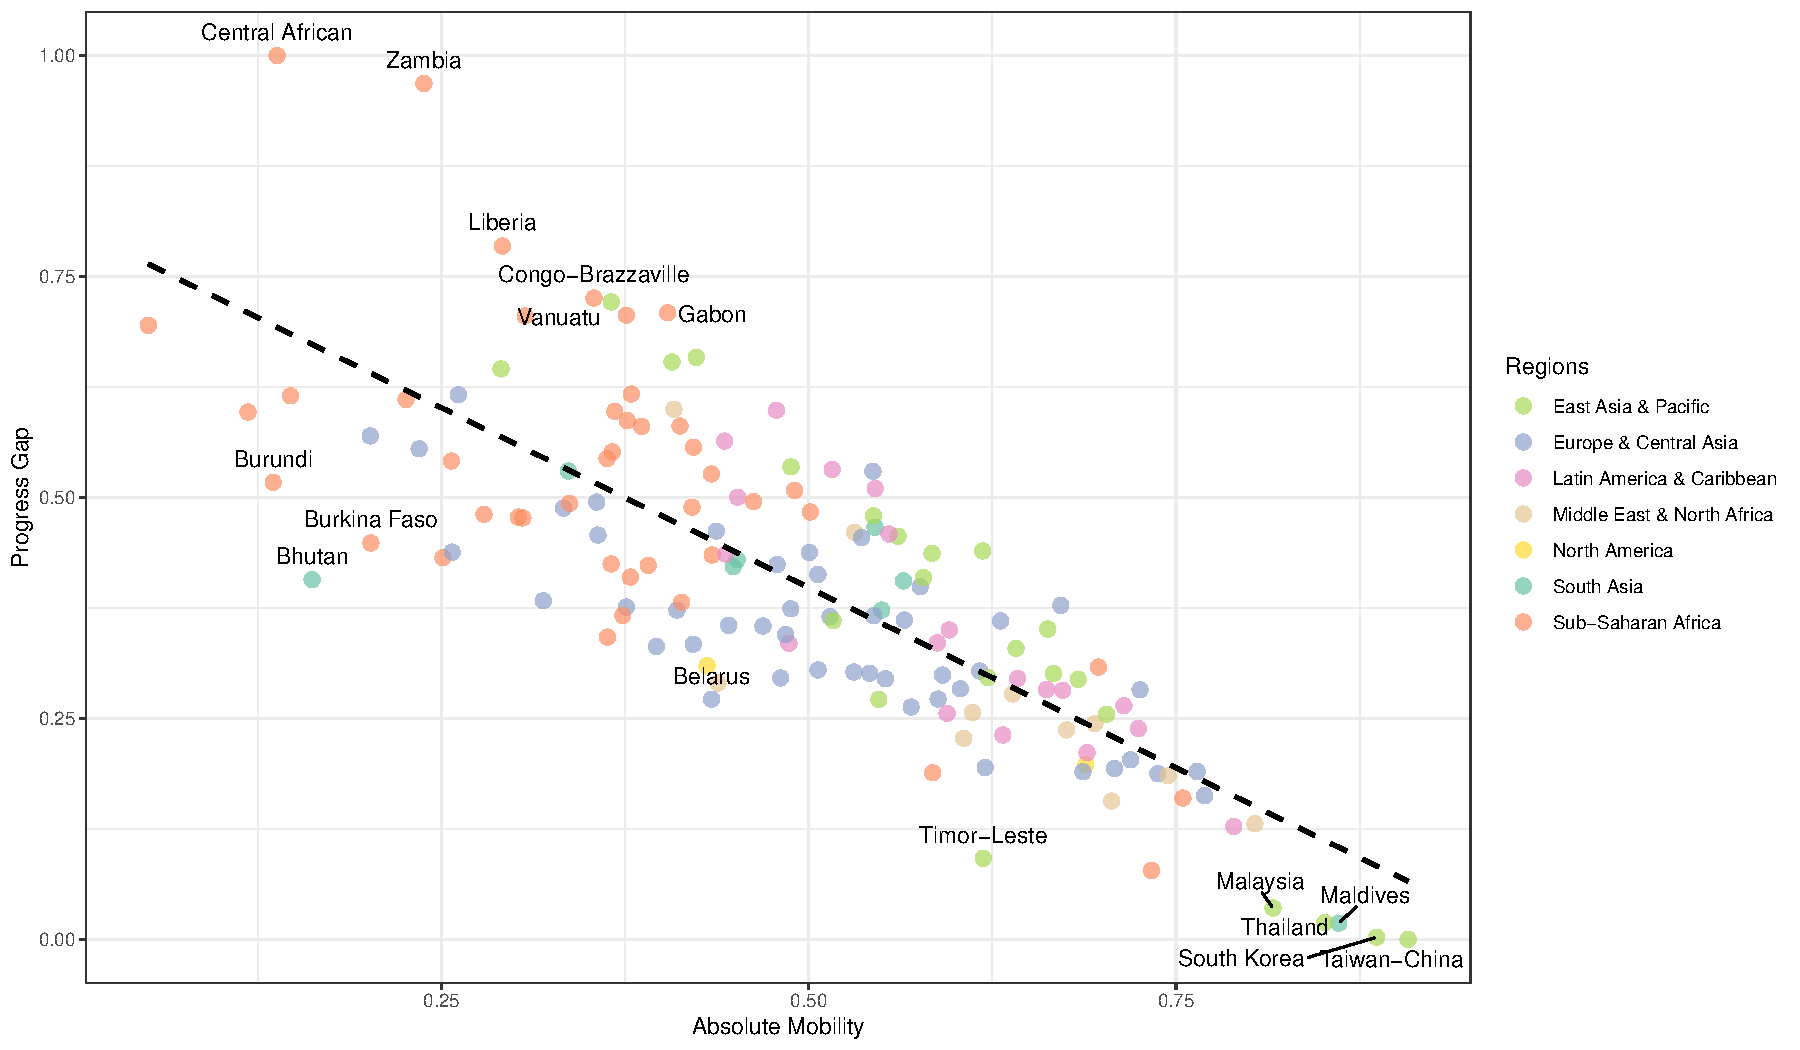
\includegraphics{figs/abs_pro2.pdf}}

\scalebox{0.5}{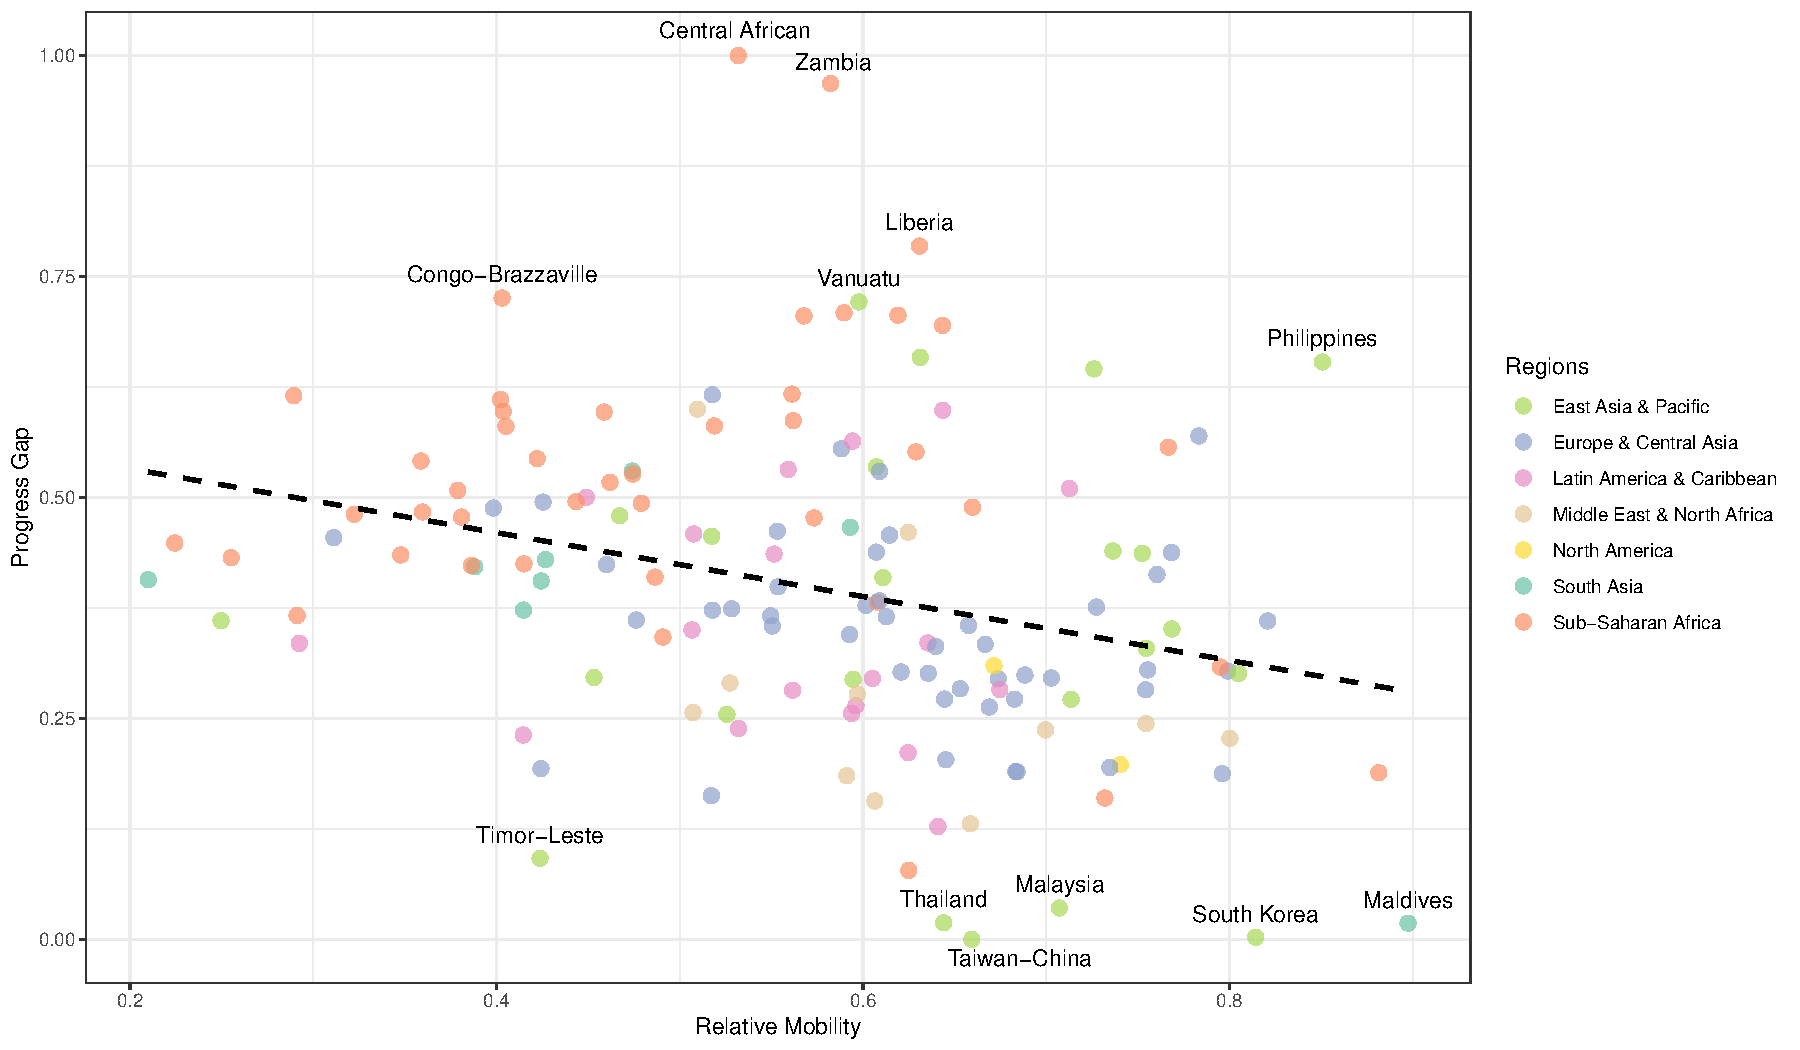
\includegraphics{figs/rel_pro2.pdf}}





